\documentclass[11pt,a4paper]{article}

% =========================================================
% Packages
% =========================================================
\usepackage[margin=2.2cm]{geometry}
\usepackage{graphicx}
\usepackage{xcolor}
\usepackage{hyperref}
\usepackage{array}
\usepackage{booktabs}
\usepackage{tabularx}
\usepackage{longtable}
\usepackage{fancyhdr}
\usepackage{lastpage}
\usepackage{fontspec}
\usepackage{setspace}
\usepackage{tikz}
\usepackage{enumitem}
\usepackage{multicol}
\usepackage{tcolorbox}
\usepackage{float}
\usepackage{amssymb}
\usepackage{amsmath}
\usepackage{listings}
\usepackage{fontawesome5}
\usepackage{pifont}

\usetikzlibrary{shapes.geometric, arrows.meta, positioning, fit, backgrounds, calc, decorations.pathreplacing, shapes.symbols, shapes.misc}
\tcbuselibrary{skins, breakable}

% =========================================================
% Tollgate Brand Palette (derived from logo)
% =========================================================
\definecolor{tollgatepink}{HTML}{E6007E}
\definecolor{tollgatepinklight}{HTML}{FFE3F0}
\definecolor{tollgateblack}{HTML}{0A0A0A}
\definecolor{tollgatecharcoal}{HTML}{1F2937}
\definecolor{tollgateslate}{HTML}{2B2D42}
\definecolor{tollgatearc}{HTML}{2775CA}
\definecolor{tollgatearclight}{HTML}{E8F1FB}
\definecolor{tollgategreen}{HTML}{06A77D}
\definecolor{tollgategreenlight}{HTML}{E0F5EE}
\definecolor{tollgategold}{HTML}{F2A541}
\definecolor{tollgategoldlight}{HTML}{FDF4E3}
\definecolor{tollgategray}{HTML}{6B7280}
\definecolor{tollgategraylight}{HTML}{F3F4F6}
\definecolor{tollgatemaroon}{HTML}{7C2D3A}
\definecolor{tollgatemaroonlight}{HTML}{F9E8EC}
\definecolor{sectionbg}{HTML}{FAFAFA}
\definecolor{codebg}{HTML}{1E1E1E}
\definecolor{codetext}{HTML}{D4D4D4}

% =========================================================
% Fonts
% =========================================================
\setmainfont{Calibri}
\setmonofont{Consolas}

% =========================================================
% Custom column types
% =========================================================
\newcolumntype{L}[1]{>{\raggedright\arraybackslash}p{#1}}
\newcolumntype{C}[1]{>{\centering\arraybackslash}p{#1}}
\newcolumntype{R}[1]{>{\raggedleft\arraybackslash}p{#1}}
\newcolumntype{Y}{>{\raggedright\arraybackslash}X}

% =========================================================
% Code listing style
% =========================================================
\lstdefinestyle{tollgatecode}{
  backgroundcolor=\color{codebg},
  basicstyle=\ttfamily\small\color{codetext},
  breaklines=true,
  captionpos=b,
  keepspaces=true,
  showspaces=false,
  showstringspaces=false,
  frame=none,
  xleftmargin=4mm,
  xrightmargin=4mm,
  aboveskip=3mm,
  belowskip=3mm
}
\lstset{style=tollgatecode}

% =========================================================
% Custom tcolorboxes (one per semantic category)
% =========================================================
\newtcolorbox{tollbox}[1][]{
  enhanced, colback=tollgatepinklight, colframe=tollgatepink,
  fonttitle=\bfseries\normalsize\color{tollgatecharcoal},
  coltitle=tollgatecharcoal, colbacktitle=tollgatepink!20,
  attach boxed title to top left={yshift=-2mm, xshift=5mm},
  boxed title style={sharp corners, boxrule=0pt},
  sharp corners, boxrule=1pt, top=4mm, bottom=4mm, left=4mm, right=4mm,
  before skip=6mm, after skip=6mm, #1
}

\newtcolorbox{archbox}[1][]{
  enhanced, colback=tollgatearclight, colframe=tollgatearc,
  fonttitle=\bfseries\normalsize\color{tollgatecharcoal},
  coltitle=tollgatecharcoal, colbacktitle=tollgatearc!20,
  attach boxed title to top left={yshift=-2mm, xshift=5mm},
  boxed title style={sharp corners, boxrule=0pt},
  sharp corners, boxrule=1pt, top=4mm, bottom=4mm, left=4mm, right=4mm,
  before skip=6mm, after skip=6mm, #1
}

\newtcolorbox{flowbox}[1][]{
  enhanced, colback=tollgategreenlight, colframe=tollgategreen,
  fonttitle=\bfseries\normalsize\color{tollgatecharcoal},
  coltitle=tollgatecharcoal, colbacktitle=tollgategreen!25,
  attach boxed title to top left={yshift=-2mm, xshift=5mm},
  boxed title style={sharp corners, boxrule=0pt},
  sharp corners, boxrule=1pt, top=4mm, bottom=4mm, left=4mm, right=4mm,
  before skip=6mm, after skip=6mm, #1
}

\newtcolorbox{warnbox}[1][]{
  enhanced, colback=tollgatemaroonlight, colframe=tollgatemaroon,
  fonttitle=\bfseries\normalsize\color{tollgatecharcoal},
  coltitle=tollgatecharcoal, colbacktitle=tollgatemaroon!20,
  attach boxed title to top left={yshift=-2mm, xshift=5mm},
  boxed title style={sharp corners, boxrule=0pt},
  sharp corners, boxrule=1pt, top=4mm, bottom=4mm, left=4mm, right=4mm,
  before skip=6mm, after skip=6mm, #1
}

\newtcolorbox{highlightbox}[1][]{
  enhanced, colback=tollgategoldlight, colframe=tollgategold,
  fonttitle=\bfseries\normalsize\color{tollgatecharcoal},
  coltitle=tollgatecharcoal, colbacktitle=tollgategold!25,
  attach boxed title to top left={yshift=-2mm, xshift=5mm},
  boxed title style={sharp corners, boxrule=0pt},
  sharp corners, boxrule=1pt, top=4mm, bottom=4mm, left=4mm, right=4mm,
  before skip=6mm, after skip=6mm, #1
}

% =========================================================
% Table spacing
% =========================================================
\renewcommand{\arraystretch}{1.3}

% =========================================================
% Header and Footer
% =========================================================
\pagestyle{fancy}
\fancyhf{}
\fancyhead[L]{\small\color{tollgatecharcoal}Tollgate System Architecture v1.0}
\fancyhead[R]{\small\color{tollgatecharcoal}tollgate.brianmwai.com}
\fancyfoot[C]{\small\color{tollgatecharcoal}Page \thepage\ of \pageref{LastPage}}
\renewcommand{\headrulewidth}{0.4pt}
\renewcommand{\footrulewidth}{0.4pt}

% =========================================================
% Hyperref
% =========================================================
\hypersetup{
  colorlinks=true,
  linkcolor=tollgatepink,
  urlcolor=tollgatearc,
  citecolor=tollgategreen
}

% =========================================================
% Icon shortcuts (fontawesome5; Phosphor equivalents available)
% =========================================================
\newcommand{\iconGate}{\textcolor{tollgatepink}{\faDoorOpen}}
\newcommand{\iconBot}{\textcolor{tollgateslate}{\faRobot}}
\newcommand{\iconWallet}{\textcolor{tollgategreen}{\faWallet}}
\newcommand{\iconCoin}{\textcolor{tollgategold}{\faCoins}}
\newcommand{\iconShield}{\textcolor{tollgatearc}{\faLock}}
\newcommand{\iconNetwork}{\textcolor{tollgatearc}{\faNetworkWired}}
\newcommand{\iconCloud}{\textcolor{tollgateslate}{\faCloud}}
\newcommand{\iconCode}{\textcolor{tollgateslate}{\faCode}}
\newcommand{\iconBolt}{\textcolor{tollgatepink}{\faBolt}}
\newcommand{\iconCheck}{\textcolor{tollgategreen}{\faCheckCircle}}
\newcommand{\iconChart}{\textcolor{tollgatearc}{\faChartLine}}
\newcommand{\iconKey}{\textcolor{tollgategold}{\faKey}}
\newcommand{\iconStar}{\textcolor{tollgategold}{\faStar}}
\newcommand{\iconCog}{\textcolor{tollgateslate}{\faCog}}
\newcommand{\iconGlobe}{\textcolor{tollgatearc}{\faGlobe}}

\begin{document}

% =========================================================
% TITLE PAGE
% =========================================================
\begin{titlepage}
  \centering
  \vspace*{0.6cm}

  \includegraphics[width=0.32\textwidth]{"Tollgate logo".png}

  \vspace{0.4cm}

  {\LARGE\color{tollgateblack}\textbf{System Architecture}\par}

  \vspace{0.25cm}

  {\Large\color{tollgatecharcoal} Bot-Economics Payment Infrastructure on Arc\par}

  \vspace{0.15cm}

  {\large\color{tollgategray}\itshape Cloudflare for AI bots that pays publishers instead of blocking them.\par}

  \vspace{0.7cm}

  % Tagline box
  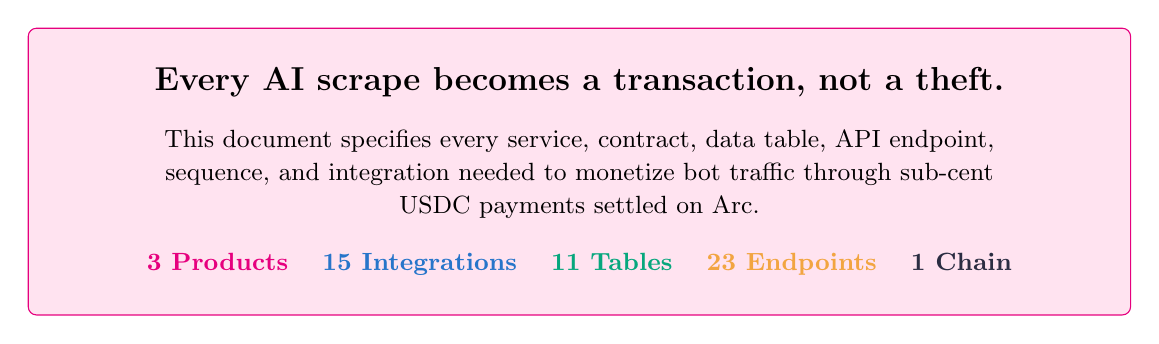
\begin{tikzpicture}
    \node[draw=tollgatepink, fill=tollgatepinklight, rounded corners=3pt, minimum width=14cm, minimum height=3.2cm, align=center, inner sep=5mm] {
      \large\textbf{Every AI scrape becomes a transaction, not a theft.}\\[3mm]
      \small This document specifies every service, contract, data table, API endpoint,\\
      \small sequence, and integration needed to monetize bot traffic through sub-cent\\
      \small USDC payments settled on Arc.\\[3mm]
      \small
        \textcolor{tollgatepink}{\textbf{3 Products}} \quad
        \textcolor{tollgatearc}{\textbf{15 Integrations}} \quad
        \textcolor{tollgategreen}{\textbf{11 Tables}} \quad
        \textcolor{tollgategold}{\textbf{23 Endpoints}} \quad
        \textcolor{tollgateslate}{\textbf{1 Chain}}
    };
  \end{tikzpicture}

  \vspace{0.6cm}

  % Journey diagram: request lifecycle
  
\begin{tikzpicture}[
    pstep/.style={draw, rounded corners=3pt, minimum width=2.1cm, minimum height=1.2cm, align=center, font=\scriptsize, inner sep=1.3mm},
    arr/.style={-stealth, thick, tollgatepink}
  ]
    \node[pstep, fill=tollgategraylight, draw=tollgateslate] (a) at (0,0) {\textbf{BOT REQ}\\GET /article};
    \node[pstep, fill=tollgatepinklight, draw=tollgatepink] (b) at (2.5,0) {\textbf{402}\\Pay Required};
    \node[pstep, fill=tollgategoldlight, draw=tollgategold] (c) at (5,0) {\textbf{SIGN}\\Arc TX};
    \node[pstep, fill=tollgatearclight, draw=tollgatearc] (d) at (7.5,0) {\textbf{VERIFY}\\x402 Facilitator};
    \node[pstep, fill=tollgategreenlight, draw=tollgategreen] (e) at (10,0) {\textbf{SERVE}\\200 + Content};
    \node[pstep, fill=tollgategreenlight, draw=tollgategreen] (f) at (12.5,0) {\textbf{EARN}\\USDC Credit};
    \draw[arr] (a) -- (b);
    \draw[arr] (b) -- (c);
    \draw[arr] (c) -- (d);
    \draw[arr] (d) -- (e);
    \draw[arr] (e) -- (f);
  \end{tikzpicture}

  \vfill

  {\normalsize\color{tollgatecharcoal}\textbf{Version:} 1.0 \quad \textbf{Date:} April 2026 \quad \textbf{Classification:} Hackathon Submission / Public\par}
  \vspace{0.2cm}
  {\small\textbf{Author:} Brian Mwai \quad \textbf{Built for:} Agentic Economy on Arc -- Circle Hackathon, SF, 2026\par}
  \vspace{0.1cm}
  {\footnotesize\color{tollgategray}github.com/brn-mwai/tollgate \quad $\diamond$ \quad tollgate.brianmwai.com\par}

\end{titlepage}

% =========================================================
% TABLE OF CONTENTS
% =========================================================
\tableofcontents
\newpage

%===============================================================================
% SECTION 0: DOCUMENT PREFACE
%===============================================================================
\section*{Preface}
\addcontentsline{toc}{section}{Preface}

\begin{tollbox}[title={\iconGate~ What this document is}]
This is the \textbf{complete system architecture} for Tollgate, a payment rail that lets web publishers charge AI bots a fraction of a cent per request in USDC, settled on Arc with sub-second finality.

It follows a seven-step design framework: \textbf{Clarify} requirements, \textbf{Estimate} capacity, \textbf{Architect} the high-level system, \textbf{Detail} workflows, \textbf{Design} APIs and schema, \textbf{Scale} along a growth path, and \textbf{Verify} that non-functional requirements are met by concrete design decisions.

Every box, table, and diagram in this document is justified by a requirement. Every external call is isolated in an action. Every query has an index. This is a build specification, not a pitch deck.
\end{tollbox}

\begin{highlightbox}[title={\iconStar~ The single sentence we repeat}]
\centering
\large\itshape Tollgate turns every AI scraper request from a theft into a transaction.
\end{highlightbox}

\newpage

%===============================================================================
% SECTION 1: CLARIFY
%===============================================================================
\section{Clarify: Requirements}

\begin{archbox}[title={\iconCog~ Context answered first}]
\textbf{User roles.} Publisher (website owner), Agent (AI bot operator), Admin (Tollgate staff).

\textbf{DAU targets.} Launch: 100 publishers $\times$ 50 agents $\approx$ 5K DAU. Year 1: 10K publishers $\times$ 1K agents $\approx$ 500K DAU. Year 3: 100K publishers $\times$ 50K agents $\approx$ 5M DAU.

\textbf{Workload profile.} Heavily write-heavy. Each request produces one to three database writes. Read-to-write ratio sits near 1:20, which pushes the design toward materialized rollups rather than live aggregation.

\textbf{Regulated data.} No PII on agents (wallet address is the only identifier). Publishers are KYCd through Circle Wallets. Every onchain transaction is public by design. Tollgate never touches money transmission: the publisher is the merchant of record, Tollgate is the SaaS that sits between.
\end{archbox}

\subsection{Functional Requirements}

\begin{table}[H]
\centering
\footnotesize
\begin{tabularx}{\textwidth}{@{} l X @{}}
\toprule
\textbf{ID} & \textbf{Requirement} \\
\midrule
F-01 & Publisher can sign up, verify site ownership, install middleware via SDK or hosted Worker. \\
F-02 & Publisher configures per-path pricing, bot whitelists, blacklists, and reputation tiers. \\
F-03 & Publisher receives a programmable Circle Wallet on Arc at onboarding. No key management required. \\
F-04 & Middleware returns HTTP 402 for unpaid bot requests, with price, nonce, recipient, chain, and expiry. \\
F-05 & Agent SDK auto-detects 402, signs USDC transfer on Arc, retries request with payment proof. \\
F-06 & Middleware verifies proof via x402 facilitator and serves content on success. \\
F-07 & Middleware issues short-TTL HMAC receipts so repeat requests skip onchain round-trip. \\
F-08 & Control plane aggregates events in real time and streams live earnings to the publisher dashboard. \\
F-09 & Publisher can withdraw USDC to any chain via Circle CCTP and off-ramp to bank. \\
F-10 & Agents accrue onchain reputation via ERC-8004 contract, feeding tiered discount pricing. \\
F-11 & Admin can suspend abusive wallets, moderate disputes, and view network-wide health. \\
F-12 & Agents can query AIsa Nanopayment APIs through the same SDK flow for upstream data needs. \\
\bottomrule
\end{tabularx}
\end{table}

\subsection{Non-Functional Requirements}

\begin{table}[H]
\centering
\footnotesize
\begin{tabularx}{\textwidth}{@{} l l X @{}}
\toprule
\textbf{NFR} & \textbf{Target} & \textbf{Rationale} \\
\midrule
Availability (middleware) & 99.99\% & Publisher sites must not go down because of Tollgate. \\
Availability (control plane) & 99.95\% & Dashboard outage tolerable; payments must keep flowing. \\
p95 latency (cached request) & $<$ 50 ms & Receipt path must feel invisible to scrapers. \\
p95 latency (cold request) & $<$ 1.2 s & First payment: 402 round-trip + Arc sign + facilitator verify. \\
Consistency (wallet balance) & Strong & Circle Wallets as source of truth; reconcile nightly. \\
Consistency (analytics) & Eventual & Batched 5s ingest; hourly rollups; publisher accepts lag. \\
Throughput target (Y3) & 10K req/s sustained, 50K peak & Network-effect driven scale curve. \\
Compliance & SOC 2 Type II by Y1 & Enterprise publisher sales gate. \\
Privacy & GDPR / CCPA for publishers & Agents are pseudonymous by protocol. \\
Security & Nonce replay, signature, HMAC & Standard for payment systems + x402 spec. \\
\bottomrule
\end{tabularx}
\end{table}

\subsection{Out of Scope}

\begin{itemize}[leftmargin=*]
  \item Human micropayments. Bots only. Every prior micropayment startup died trying to charge humans.
  \item Fiat rails (Stripe, ACH) for payment-in. USDC only at MVP. Off-ramp is fiat-aware via Circle.
  \item Non-Arc chains at launch. Bridge Kit adds support post-MVP without changing the SDK surface.
  \item Content-level DRM. We gate access; we do not police downstream reuse.
  \item Human CAPTCHA. Publishers pass human traffic through before Tollgate sees it.
  \item Bot classification. We trust the client identifier; misuse is priced out by reputation over time.
\end{itemize}

\subsection{Assumptions}

\begin{itemize}[leftmargin=*]
  \item Publisher already runs a web server capable of hosting middleware (Express, Hono, CF Worker, Next.js, nginx sidecar).
  \item Agent operator can sign transactions programmatically, either through a self-custody Arc wallet or through Circle Wallets API.
  \item Arc testnet and mainnet are reachable via RPC. Official faucet funds demo wallets.
  \item The x402 facilitator (Coinbase-hosted at MVP, self-hosted at scale) returns verdicts in under 400 ms.
  \item Circle Wallets API provides adequate throughput for per-publisher wallet provisioning.
  \item AIsa APIs expose Nanopayment-ready endpoints that Tollgate agents can call natively.
\end{itemize}

\newpage

%===============================================================================
% SECTION 2: ESTIMATE
%===============================================================================
\section{Estimate: Capacity}

\begin{flowbox}[title={\iconChart~ Sizing the system}]
Base unit of work is the \textbf{event row}: one HTTP request to a protected path produces one event. Every other estimate derives from this.
\end{flowbox}

\subsection{Year 1 Capacity Table}

\begin{table}[H]
\centering
\footnotesize
\begin{tabularx}{\textwidth}{@{} l l X @{}}
\toprule
\textbf{Metric} & \textbf{Value} & \textbf{Formula / Notes} \\
\midrule
Daily events & 100M / day & 500K DAU $\times$ 200 req / user / day avg \\
Monthly events & 3B / month & Daily $\times$ 30 \\
Avg row size (events) & 320 B & Indexed fields + optional metadata \\
Storage, hot events (90d, 1.3 replication) & 3.7 TB & $320 \text{ B} \times 100\text{M} \times 90 \times 1.3$ \\
Ingress + egress bandwidth & 200 GB / day & $2\text{ KB} \times 100\text{M}$ \\
Peak QPS & 3.5K QPS & $(100\text{M} \times 3) / 86400$ \\
Concurrent connections & 35K & DAU $\times 0.07$ \\
Convex function calls / month & $\sim$ 6.2B & 3B events $\times$ 2 writes + 200M reads \\
Onchain TX uncached (ceiling) & $\sim$ 900M / month & 30\% miss rate without receipts \\
Onchain TX with receipts (target) & $\sim$ 30M / month & 50x collapse via 5-min HMAC receipts \\
Clerk MAU (publisher accounts) & $\sim$ 10K & Publisher seats only \\
\bottomrule
\end{tabularx}
\end{table}

\subsection{Read to Write Analysis}

\begin{archbox}[title={\iconBolt~ Design implication}]
With 6.2 billion Convex function calls per month at Year 1, running the dashboard off raw events becomes an economic hazard. The design therefore relies on:

\begin{itemize}[leftmargin=*]
  \item Edge-side batching of telemetry (5-second flush window, 100-event cap per batch).
  \item Hourly rollup tables that the dashboard reads from, not raw events.
  \item Seven-day hot retention in Convex, older events archived to Cloudflare R2.
  \item Receipt caching at the middleware layer, collapsing 50 requests into 1 onchain TX.
\end{itemize}

Without this stack of compressions, Convex billing alone becomes the dominant cost and the product becomes un-shippable. With it, control-plane cost stays well inside a healthy gross margin even at Year 1 scale.
\end{archbox}

\newpage

%===============================================================================
% SECTION 3: ARCHITECT
%===============================================================================
\section{Architect: High-Level Design}

\subsection{Six-Layer Architecture}

\begin{center}
\begin{tikzpicture}[
  x=1cm, y=1cm,
  comp/.style={draw, rounded corners=2pt, minimum width=2.9cm, minimum height=1.0cm, align=center, font=\scriptsize, inner sep=1.2mm},
  bandtitle/.style={font=\footnotesize\bfseries, anchor=north west},
  arr/.style={-stealth, very thick, tollgatecharcoal}
]

% Band 1 CLIENT
\draw[fill=tollgatepinklight!40, draw=tollgatepink, thick, rounded corners=3pt] (-7,10) rectangle (7,12);
\node[bandtitle, text=tollgatepink] at (-6.9,11.95) {CLIENT LAYER};
\node[comp, fill=tollgatepinklight, draw=tollgatepink] at (-4.8,11.0) {\iconBot~Agent SDK\\Node / Python};
\node[comp, fill=tollgategoldlight, draw=tollgategold] at (-1.6,11.0) {\iconCode~Publisher SDK\\Express / Hono / CFW};
\node[comp, fill=tollgatearclight, draw=tollgatearc] at (1.6,11.0) {\iconChart~Dashboard\\Next.js 16};
\node[comp, fill=tollgategreenlight, draw=tollgategreen] at (4.8,11.0) {\iconGlobe~Hosted Gateway\\No-Code};

% Band 2 EDGE
\draw[fill=tollgatepinklight!25, draw=tollgatepink, thick, rounded corners=3pt] (-7,7.4) rectangle (7,9.4);
\node[bandtitle, text=tollgatepink] at (-6.9,9.35) {EDGE LAYER};
\node[comp, fill=white, draw=tollgatepink] at (-4.8,8.4) {\iconGate~Tollgate\\Middleware};
\node[comp, fill=white, draw=tollgatepink] at (-1.6,8.4) {\iconShield~x402\\Facilitator};
\node[comp, fill=white, draw=tollgatepink] at (1.6,8.4) {\iconKey~HMAC\\Receipt Signer};
\node[comp, fill=white, draw=tollgatepink] at (4.8,8.4) {\iconBolt~Edge KV\\Nonce + Pricing};

% Band 3 SERVICE
\draw[fill=tollgatearclight!40, draw=tollgatearc, thick, rounded corners=3pt] (-7,4.8) rectangle (7,6.8);
\node[bandtitle, text=tollgatearc] at (-6.9,6.75) {SERVICE LAYER (CONVEX)};
\node[comp, fill=white, draw=tollgatearc] at (-4.8,5.8) {\iconCog~queries};
\node[comp, fill=white, draw=tollgatearc] at (-1.6,5.8) {\iconCog~mutations};
\node[comp, fill=white, draw=tollgatearc] at (1.6,5.8) {\iconCloud~actions};
\node[comp, fill=white, draw=tollgatearc] at (4.8,5.8) {\iconKey~httpActions\\+ cron};

% Band 4 DATA
\draw[fill=tollgategraylight, draw=tollgatecharcoal, thick, rounded corners=3pt] (-7,2.2) rectangle (7,4.2);
\node[bandtitle, text=tollgatecharcoal] at (-6.9,4.15) {DATA LAYER};
\node[comp, fill=white, draw=tollgatecharcoal] at (-4.8,3.2) {Convex DB\\11 tables};
\node[comp, fill=white, draw=tollgatecharcoal] at (-1.6,3.2) {Vector Index\\clustering};
\node[comp, fill=white, draw=tollgatecharcoal] at (1.6,3.2) {Search Index\\labels};
\node[comp, fill=white, draw=tollgatecharcoal] at (4.8,3.2) {Cloudflare R2\\cold events};

% Band 5 ONCHAIN
\draw[fill=tollgategoldlight!60, draw=tollgategold, thick, rounded corners=3pt] (-7,-0.4) rectangle (7,1.6);
\node[bandtitle, text=tollgategold!80!black] at (-6.9,1.55) {ONCHAIN (ARC L1)};
\node[comp, fill=white, draw=tollgategold] at (-3.4,0.6) {\iconNetwork~Arc RPC};
\node[comp, fill=white, draw=tollgategold] at (0,0.6) {\iconCoin~USDC (native gas)};
\node[comp, fill=white, draw=tollgategold] at (3.4,0.6) {\iconStar~ERC-8004\\Reputation};

% Band 6 EXTERNAL
\draw[fill=tollgategreenlight!50, draw=tollgategreen, thick, rounded corners=3pt] (-7,-3) rectangle (7,-1);
\node[bandtitle, text=tollgategreen!70!black] at (-6.9,-1.05) {EXTERNAL SERVICES};
\node[comp, fill=white, draw=tollgategreen] at (-5.0,-2) {Circle Wallets};
\node[comp, fill=white, draw=tollgategreen] at (-2.0,-2) {Circle Gateway};
\node[comp, fill=white, draw=tollgategreen] at (1.0,-2) {Circle CCTP};
\node[comp, fill=white, draw=tollgategreen] at (4.0,-2) {AIsa + Clerk};

% Connecting arrows between bands (two per gap, offset left and right)
\draw[arr] (-3.5,10) -- (-3.5,9.4);
\draw[arr] (3.5,10) -- (3.5,9.4);
\draw[arr] (-3.5,7.4) -- (-3.5,6.8);
\draw[arr] (3.5,7.4) -- (3.5,6.8);
\draw[arr] (-3.5,4.8) -- (-3.5,4.2);
\draw[arr] (3.5,4.8) -- (3.5,4.2);
\draw[arr] (-3.5,2.2) -- (-3.5,1.6);
\draw[arr] (3.5,2.2) -- (3.5,1.6);
\draw[arr] (-3.5,-0.4) -- (-3.5,-1);
\draw[arr] (3.5,-0.4) -- (3.5,-1);

\end{tikzpicture}
\end{center}

\textbf{Reading this diagram.} Top to bottom, data and trust flow downward: clients issue requests, the edge handles gating and payment verification, Convex holds application state, data layer persists, onchain settles, external services provide value. Each band can scale independently because responsibilities are cleanly separated.

\subsection{Component Responsibilities}

\begin{table}[H]
\centering
\footnotesize
\begin{tabularx}{\textwidth}{@{} l X l @{}}
\toprule
\textbf{Component} & \textbf{Responsibility \& why chosen} & \textbf{Rejected alternative} \\
\midrule
Middleware SDK & Runs in publisher process for lowest latency. One-line install. & DNS-level proxy: adds hop, violates permissionless positioning. \\
Hosted Gateway & Managed Cloudflare Worker for non-technical publishers (WordPress, Ghost). & Plugin-only: excludes long-tail, caps growth. \\
Convex Functions & Reactive reads, transactional writes, vector, cron, file storage in one platform. & Postgres + Redis + Kafka: three systems, no reactivity, higher ops burden. \\
x402 Facilitator & Onchain proof verification + nonce dedup + caching. Coinbase-hosted at MVP. & DIY verify: no dedup, no cache, duplicated effort across deployments. \\
Arc L1 & Settlement layer. USDC-denominated gas gives deterministic margin math. & Ethereum / Polygon / Base: volatile gas destroys sub-cent unit economics. \\
Circle Wallets & Publisher custody abstraction. Zero-key onboarding. & Self-custody wallet: kills publisher conversion at signup. \\
Circle Gateway & Agent-side unified USDC across chains. One integration, any chain. & Per-chain wallet config: agent operators refuse integration complexity. \\
Circle Bridge Kit & Publisher off-ramp to Base / Ethereum then to bank. & Manual bridging: dashboard UX breaks. \\
ERC-8004 (Vyper) & Onchain agent reputation. Portable across networks. & Off-chain reputation DB: centralized, not portable, not agent-friendly. \\
Clerk & Publisher auth, JWT template for Convex. & Custom auth: compliance burden, no SOC 2 inheritance. \\
Cloudflare R2 & Cold event archive beyond seven days. & Convex storage: not priced for multi-TB cold data. \\
AIsa APIs & Upstream data source consumed through same Nanopayment flow. Dogfood. & Skip: loses "Tollgate as both provider and consumer" narrative. \\
\bottomrule
\end{tabularx}
\end{table}

\newpage

%===============================================================================
% SECTION 4: DETAIL
%===============================================================================
\section{Detail: Critical Workflows}

Every workflow below traces end-to-end: trigger, client call, auth check, database mutation, external call, response shape, failure mode.

\subsection{Workflow A: Publisher Onboarding}

\begin{flowbox}[title={\iconCheck~ Path A --- From Clerk signup to live middleware}]
\textbf{Trigger:} Publisher visits \texttt{tollgate.brianmwai.com} and clicks sign up.\\
\textbf{Outcome:} Publisher has a funded Circle Wallet on Arc, an active site with API key, and a one-line install snippet.
\end{flowbox}

\begin{center}
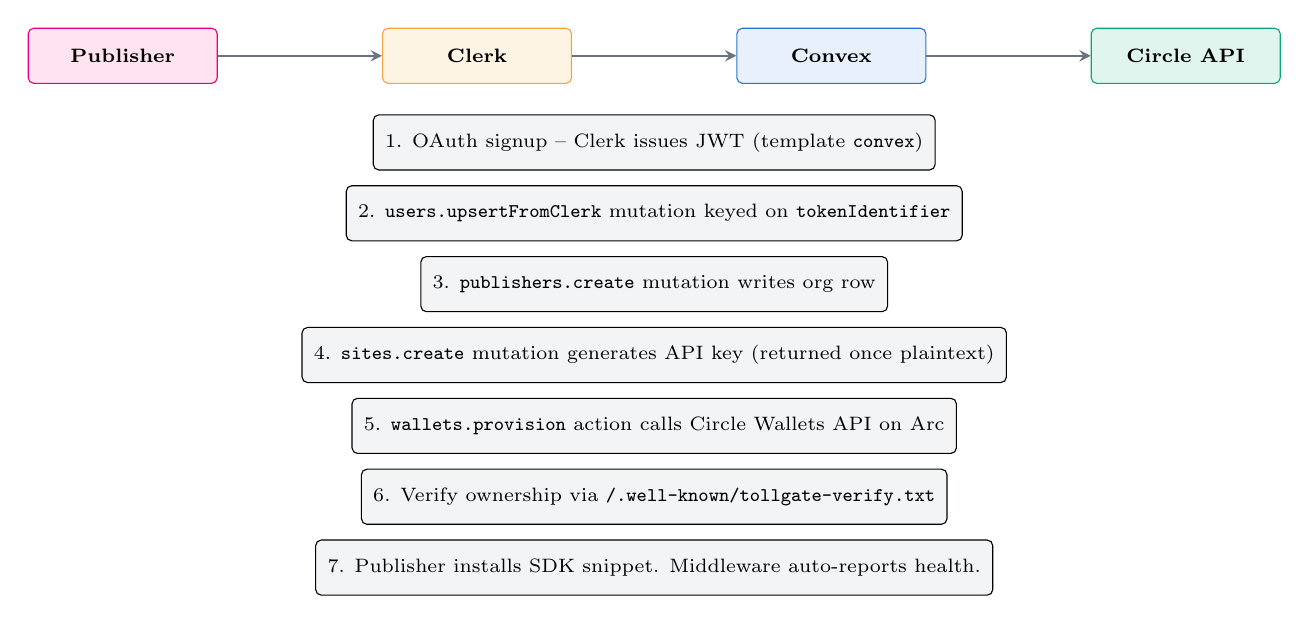
\begin{tikzpicture}[
  actor/.style={draw, rounded corners=2pt, minimum width=2.4cm, minimum height=0.7cm, align=center, font=\scriptsize, inner sep=1mm},
  action/.style={draw, rounded corners=2pt, minimum width=5.8cm, minimum height=0.7cm, align=left, font=\scriptsize, inner sep=1.5mm, fill=tollgategraylight},
  arrow/.style={-stealth, thick}
]
\node[actor, fill=tollgatepinklight, draw=tollgatepink] (u) at (0,0) {\textbf{Publisher}};
\node[actor, fill=tollgategoldlight, draw=tollgategold] (c) at (4.5,0) {\textbf{Clerk}};
\node[actor, fill=tollgatearclight, draw=tollgatearc] (cv) at (9,0) {\textbf{Convex}};
\node[actor, fill=tollgategreenlight, draw=tollgategreen] (ci) at (13.5,0) {\textbf{Circle API}};

\node[action] (a1) at (6.75,-1.1) {1. OAuth signup -- Clerk issues JWT (template \texttt{convex})};
\node[action] (a2) at (6.75,-2.0) {2. \texttt{users.upsertFromClerk} mutation keyed on \texttt{tokenIdentifier}};
\node[action] (a3) at (6.75,-2.9) {3. \texttt{publishers.create} mutation writes org row};
\node[action] (a4) at (6.75,-3.8) {4. \texttt{sites.create} mutation generates API key (returned once plaintext)};
\node[action] (a5) at (6.75,-4.7) {5. \texttt{wallets.provision} action calls Circle Wallets API on Arc};
\node[action] (a6) at (6.75,-5.6) {6. Verify ownership via \texttt{/.well-known/tollgate-verify.txt}};
\node[action] (a7) at (6.75,-6.5) {7. Publisher installs SDK snippet. Middleware auto-reports health.};

\draw[arrow, tollgategray] (u) -- (c);
\draw[arrow, tollgategray] (c) -- (cv);
\draw[arrow, tollgategray] (cv) -- (ci);
\end{tikzpicture}
\end{center}

\textbf{Failure modes.} Circle API timeout: retry three times with exponential backoff, queue via \texttt{ctx.scheduler.runAfter}. Ownership file missing: site stays \texttt{unverified}, 402 disabled, publisher prompted with exact remediation.

\subsection{Workflow B: Paid Agent Request (Cold, Uncached)}

\begin{flowbox}[title={\iconBolt~ Path B --- 402 to 200 in under one second}]
\textbf{Trigger:} AI agent issues GET to a protected path with no payment header.\\
\textbf{Outcome:} One onchain USDC TX, one content delivery, one event recorded, one receipt issued.
\end{flowbox}

\begin{center}
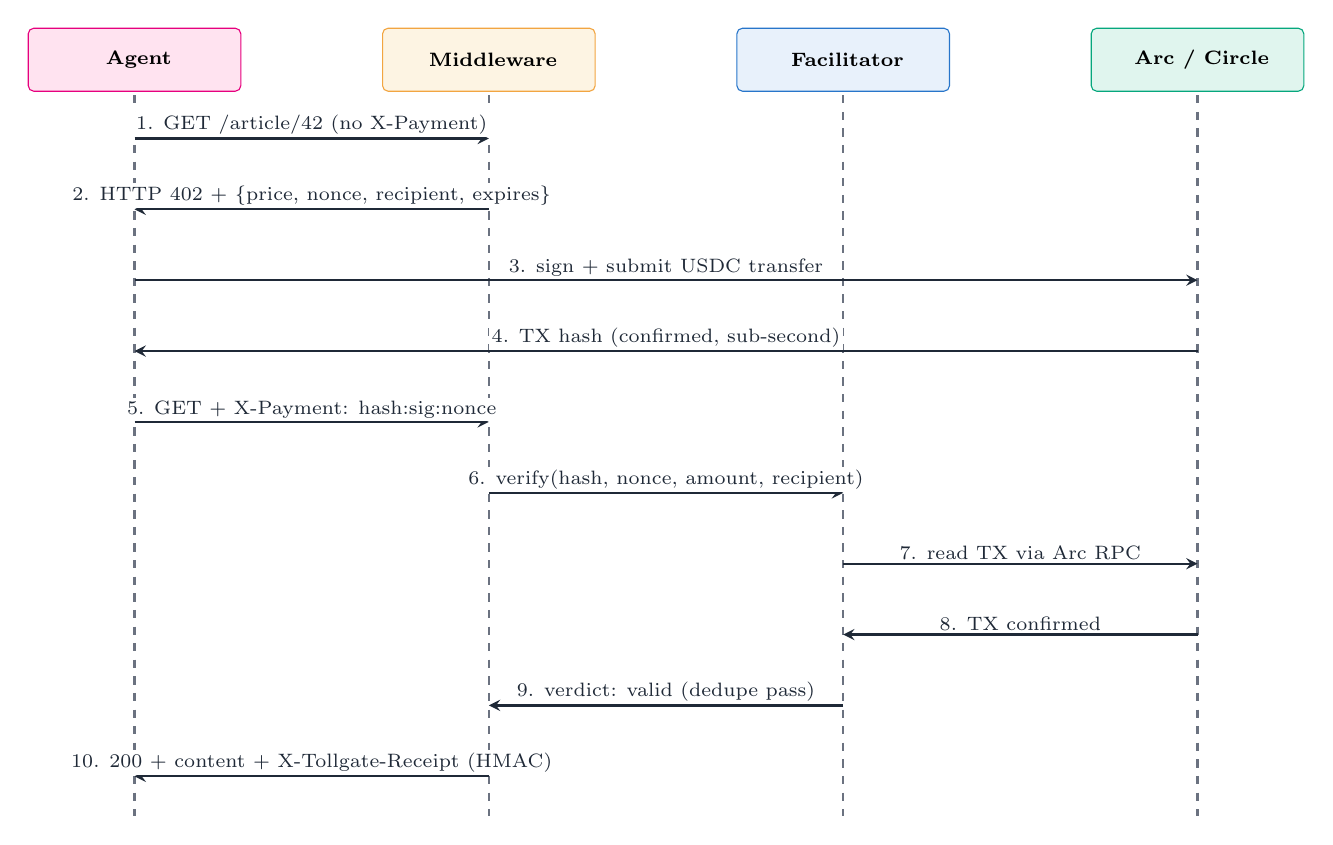
\begin{tikzpicture}[
  x=1cm, y=1cm,
  actor/.style={draw, rounded corners=2pt, minimum width=2.7cm, minimum height=0.8cm, align=center, font=\scriptsize\bfseries, inner sep=1mm},
  lifeline/.style={dashed, tollgategray, thick},
  msg/.style={-stealth, thick, tollgatecharcoal},
  mlabel/.style={font=\scriptsize, fill=white, inner sep=1pt}
]
% Actors
\node[actor, fill=tollgatepinklight, draw=tollgatepink] (ag) at (0,0) {\iconBot~Agent};
\node[actor, fill=tollgategoldlight, draw=tollgategold] (mw) at (4.5,0) {\iconGate~Middleware};
\node[actor, fill=tollgatearclight, draw=tollgatearc] (fc) at (9,0) {\iconShield~Facilitator};
\node[actor, fill=tollgategreenlight, draw=tollgategreen] (arnet) at (13.5,0) {\iconNetwork~Arc / Circle};

% Lifelines
\draw[lifeline] (0,-0.45) -- (0,-9.6);
\draw[lifeline] (4.5,-0.45) -- (4.5,-9.6);
\draw[lifeline] (9,-0.45) -- (9,-9.6);
\draw[lifeline] (13.5,-0.45) -- (13.5,-9.6);

% Messages (numbered, proper arrows)
\draw[msg] (0,-1.0) -- (4.5,-1.0) node[mlabel, midway, above] {1. GET /article/42 (no X-Payment)};
\draw[msg] (4.5,-1.9) -- (0,-1.9) node[mlabel, midway, above] {2. HTTP 402 + \{price, nonce, recipient, expires\}};
\draw[msg] (0,-2.8) -- (13.5,-2.8) node[mlabel, midway, above] {3. sign + submit USDC transfer};
\draw[msg] (13.5,-3.7) -- (0,-3.7) node[mlabel, midway, above] {4. TX hash (confirmed, sub-second)};
\draw[msg] (0,-4.6) -- (4.5,-4.6) node[mlabel, midway, above] {5. GET + X-Payment: hash:sig:nonce};
\draw[msg] (4.5,-5.5) -- (9,-5.5) node[mlabel, midway, above] {6. verify(hash, nonce, amount, recipient)};
\draw[msg] (9,-6.4) -- (13.5,-6.4) node[mlabel, midway, above] {7. read TX via Arc RPC};
\draw[msg] (13.5,-7.3) -- (9,-7.3) node[mlabel, midway, above] {8. TX confirmed};
\draw[msg] (9,-8.2) -- (4.5,-8.2) node[mlabel, midway, above] {9. verdict: valid (dedupe pass)};
\draw[msg] (4.5,-9.1) -- (0,-9.1) node[mlabel, midway, above] {10. 200 + content + X-Tollgate-Receipt (HMAC)};

\end{tikzpicture}
\end{center}

\textbf{Failure modes.} Facilitator timeout beyond five seconds: fall through to fail-open if publisher opts in, otherwise another 402. Signature mismatch: reject with fresh nonce. Double-spend: rejected by Arc, returns 402.

\subsection{Workflow C: Paid Agent Request (Warm, Cached Receipt)}

\begin{flowbox}[title={\iconStar~ Path C --- sub-50ms served request}]
\textbf{Trigger:} Agent sends GET with a valid X-Tollgate-Receipt header.\\
\textbf{Outcome:} Middleware HMAC-verifies locally. No Convex call. No facilitator call. No onchain TX. Content served.
\end{flowbox}

This collapses 50-request scrape sessions into a single onchain TX plus 49 cached hits, reducing gas spend fiftyfold at the scraper level while still allowing the publisher to settle in real time on the first request.

\subsection{Workflow D: Publisher Withdraw}

\begin{center}
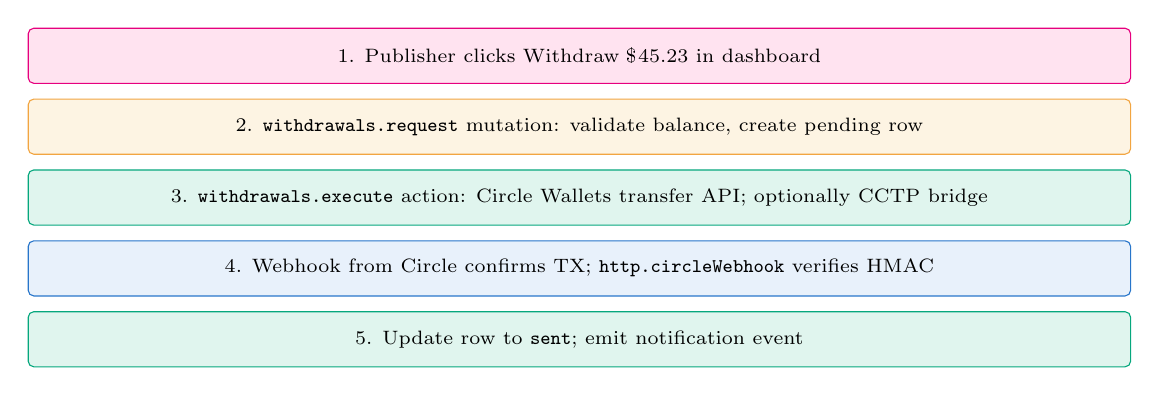
\begin{tikzpicture}[
  pstep/.style={draw, rounded corners=2pt, minimum width=14cm, minimum height=0.7cm, align=left, font=\scriptsize, inner sep=1.5mm},
  fill1/.style={fill=tollgatepinklight, draw=tollgatepink},
  fill2/.style={fill=tollgategoldlight, draw=tollgategold},
  fill3/.style={fill=tollgategreenlight, draw=tollgategreen},
  fill4/.style={fill=tollgatearclight, draw=tollgatearc}
]
\node[pstep, fill1] (w1) at (0,0) {1. Publisher clicks Withdraw \$45.23 in dashboard};
\node[pstep, fill2] (w2) at (0,-0.9) {2. \texttt{withdrawals.request} mutation: validate balance, create pending row};
\node[pstep, fill3] (w3) at (0,-1.8) {3. \texttt{withdrawals.execute} action: Circle Wallets transfer API; optionally CCTP bridge};
\node[pstep, fill4] (w4) at (0,-2.7) {4. Webhook from Circle confirms TX; \texttt{http.circleWebhook} verifies HMAC};
\node[pstep, fill3] (w5) at (0,-3.6) {5. Update row to \texttt{sent}; emit notification event};
\end{tikzpicture}
\end{center}

\textbf{Failure modes.} TX reverted: mark \texttt{failed}, refund virtual balance. Circle webhook missing: poll via scheduled function every 15 s for up to one hour.

\subsection{Workflow E: Reputation Roll-Up (Daily)}

\begin{center}
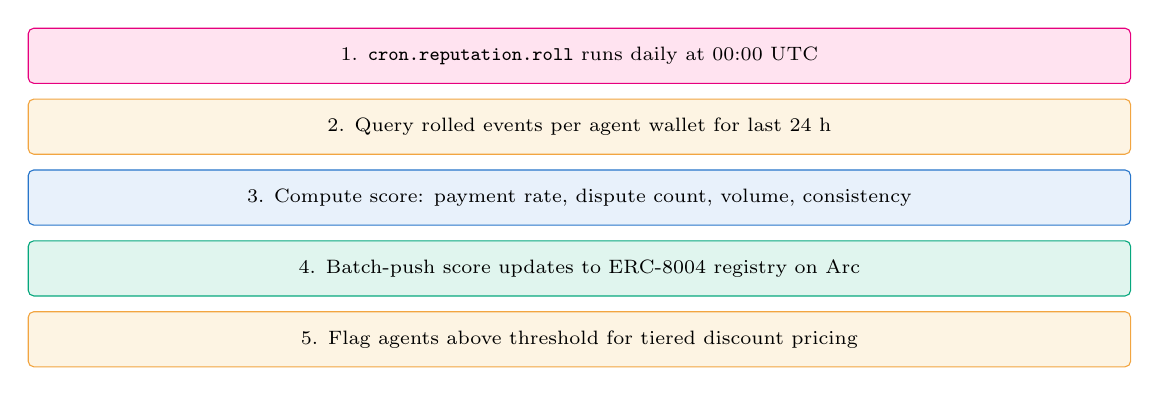
\begin{tikzpicture}[
  pstep/.style={draw, rounded corners=2pt, minimum width=14cm, minimum height=0.7cm, align=left, font=\scriptsize, inner sep=1.5mm},
  p/.style={fill=tollgatepinklight, draw=tollgatepink},
  g/.style={fill=tollgategoldlight, draw=tollgategold},
  b/.style={fill=tollgatearclight, draw=tollgatearc},
  gr/.style={fill=tollgategreenlight, draw=tollgategreen}
]
\node[pstep, p] (r1) at (0,0) {1. \texttt{cron.reputation.roll} runs daily at 00:00 UTC};
\node[pstep, g] (r2) at (0,-0.9) {2. Query rolled events per agent wallet for last 24 h};
\node[pstep, b] (r3) at (0,-1.8) {3. Compute score: payment rate, dispute count, volume, consistency};
\node[pstep, gr] (r4) at (0,-2.7) {4. Batch-push score updates to ERC-8004 registry on Arc};
\node[pstep, g] (r5) at (0,-3.6) {5. Flag agents above threshold for tiered discount pricing};
\end{tikzpicture}
\end{center}

\newpage

%===============================================================================
% SECTION 5: DESIGN
%===============================================================================
\section{Design: API and Schema}

\subsection{Convex Schema}

\begin{lstlisting}
// convex/schema.ts -- 11 tables, every query backed by an index
import { defineSchema, defineTable } from "convex/server"
import { v } from "convex/values"

export default defineSchema({
  users: defineTable({
    tokenIdentifier: v.string(),
    email: v.string(),
    name: v.optional(v.string()),
    role: v.union(v.literal("publisher"), v.literal("admin")),
  }).index("by_token", ["tokenIdentifier"])
    .index("by_email", ["email"]),

  publishers: defineTable({
    ownerId: v.id("users"),
    orgSlug: v.string(),
    plan: v.union(v.literal("free"), v.literal("pro"), v.literal("enterprise")),
    circleWalletId: v.string(),
    arcAddress: v.string(),
    balanceUsdc: v.string(),       // string for on-chain precision
    platformFeeBps: v.number(),
  }).index("by_owner", ["ownerId"])
    .index("by_slug", ["orgSlug"])
    .index("by_address", ["arcAddress"]),

  sites: defineTable({
    publisherId: v.id("publishers"),
    domain: v.string(),
    apiKeyHash: v.string(),
    status: v.union(v.literal("unverified"),
                    v.literal("active"),
                    v.literal("suspended")),
    verifyToken: v.string(),
    failOpenOnFacilitator: v.boolean(),
  }).index("by_publisher", ["publisherId"])
    .index("by_domain", ["domain"])
    .index("by_keyhash", ["apiKeyHash"]),

  pricingRules: defineTable({
    siteId: v.id("sites"),
    pathPattern: v.string(),
    priceMicroUsdc: v.number(),
    botClass: v.optional(v.string()),
    priority: v.number(),
  }).index("by_site_priority", ["siteId", "priority"]),

  agents: defineTable({
    walletAddress: v.string(),
    label: v.optional(v.string()),
    reputationScore: v.number(),
    totalPaidMicroUsdc: v.string(),
    firstSeenAt: v.number(),
    status: v.union(v.literal("active"),
                    v.literal("flagged"),
                    v.literal("banned")),
  }).index("by_wallet", ["walletAddress"])
    .index("by_score", ["reputationScore"])
    .searchIndex("search_label", { searchField: "label" }),

  events: defineTable({
    siteId: v.id("sites"),
    agentWallet: v.string(),
    path: v.string(),
    status: v.union(
      v.literal("paid_onchain"),
      v.literal("paid_cached"),
      v.literal("unpaid_402"),
      v.literal("rejected"),
      v.literal("failed_verify")
    ),
    priceMicroUsdc: v.number(),
    txHash: v.optional(v.string()),
    nonce: v.string(),
    occurredAt: v.number(),
  }).index("by_site_time", ["siteId", "occurredAt"])
    .index("by_agent_time", ["agentWallet", "occurredAt"])
    .index("by_txhash", ["txHash"])
    .index("by_nonce", ["nonce"]),

  hourlyRollup: defineTable({
    siteId: v.id("sites"),
    hourBucket: v.number(),
    totalRequests: v.number(),
    paidRequests: v.number(),
    earnedMicroUsdc: v.number(),
    uniqueAgents: v.number(),
  }).index("by_site_hour", ["siteId", "hourBucket"]),

  withdrawals: defineTable({
    publisherId: v.id("publishers"),
    amountMicroUsdc: v.string(),
    destination: v.string(),
    status: v.union(v.literal("pending"),
                    v.literal("sent"),
                    v.literal("failed")),
    circleTxId: v.optional(v.string()),
    requestedAt: v.number(),
  }).index("by_publisher_time", ["publisherId", "requestedAt"]),

  receipts: defineTable({
    hmacKey: v.string(),
    siteId: v.id("sites"),
    rotatedAt: v.number(),
  }).index("by_site", ["siteId"]),

  nonceLog: defineTable({
    nonce: v.string(),
    siteId: v.id("sites"),
    seenAt: v.number(),
  }).index("by_nonce", ["nonce"]),

  auditLog: defineTable({
    actor: v.string(),
    action: v.string(),
    entity: v.string(),
    entityId: v.string(),
    meta: v.any(),
    occurredAt: v.number(),
  }).index("by_actor_time", ["actor", "occurredAt"])
    .index("by_entity_time", ["entity", "entityId", "occurredAt"]),
})
\end{lstlisting}

\subsection{Function Surface}

\begin{table}[H]
\centering
\footnotesize
\begin{tabularx}{\textwidth}{@{} l l l X @{}}
\toprule
\textbf{Function} & \textbf{Type} & \textbf{Auth} & \textbf{Purpose} \\
\midrule
\texttt{users.upsertFromClerk} & mutation & Clerk & Upsert identity keyed on \texttt{tokenIdentifier}. \\
\texttt{publishers.create} & mutation & user & Create publisher org row. \\
\texttt{publishers.get} & query & user & Return current user's publisher record. \\
\texttt{sites.create} & mutation & publisher & Create site, generate API key, return plaintext once. \\
\texttt{sites.list} & query & publisher & Paginated site list. \\
\texttt{sites.verify} & action & publisher & Fetch \texttt{/.well-known} and confirm ownership. \\
\texttt{sites.rotateKey} & mutation & publisher & Rotate API key, log action. \\
\texttt{pricingRules.upsert} & mutation & publisher & Add or update price per path or bot class. \\
\texttt{pricingRules.list} & query & publisher & Return rules for a site. \\
\texttt{wallets.provision} & action & publisher & Call Circle Wallets API, store wallet. \\
\texttt{wallets.balance} & action & publisher & Read Arc + Circle balances. \\
\texttt{withdrawals.request} & mutation & publisher & Create pending withdrawal row. \\
\texttt{withdrawals.execute} & action & internal & Execute Circle transfer; optionally CCTP bridge. \\
\texttt{events.ingestBatch} & internalMutation & gateway & Batch-insert from edge. \\
\texttt{events.listForSite} & query & publisher & Paginated event log. \\
\texttt{hourlyRollup.forSite} & query & publisher & Dashboard time-series. \\
\texttt{agents.lookup} & query & public & Price lookup for middleware. \\
\texttt{reputation.pushOnchain} & action & internal & Batch-write ERC-8004 scores. \\
\texttt{cron.reputation.roll} & scheduled & system & Daily reputation update. \\
\texttt{cron.rollupHourly} & scheduled & system & Hourly aggregation. \\
\texttt{cron.cleanupNonces} & scheduled & system & Trim nonceLog every 10 minutes. \\
\texttt{cron.archiveColdEvents} & scheduled & system & Daily archive to R2. \\
\texttt{http.circleWebhook} & httpAction & HMAC & Receive Circle callbacks. \\
\texttt{http.telemetryIngest} & httpAction & API key & Edge batches events via this endpoint. \\
\bottomrule
\end{tabularx}
\end{table}

\subsection{Client APIs}

\begin{table}[H]
\centering
\footnotesize
\begin{tabularx}{\textwidth}{@{} l l X @{}}
\toprule
\textbf{Endpoint} & \textbf{Method} & \textbf{Purpose} \\
\midrule
\texttt{/.well-known/tollgate.json} & GET & Publisher site advertises pricing config. \\
\texttt{/v1/verify} & POST & Facilitator verifies payment proof. \\
\texttt{/v1/telemetry} & POST & Edge gateway ingests event batches. \\
\texttt{/v1/pricing} & GET & Agent-class lookup for dynamic pricing. \\
\texttt{/v1/receipts/rotate} & POST & Admin rotation of HMAC keys. \\
\texttt{/webhooks/circle} & POST & Circle callbacks (HMAC-signed). \\
\texttt{/webhooks/clerk} & POST & Clerk lifecycle webhooks. \\
\bottomrule
\end{tabularx}
\end{table}

\newpage

%===============================================================================
% SECTION 6: SCALE
%===============================================================================
\section{Scale: Growth Path}

\begin{flowbox}[title={\iconChart~ Four stages from 0 to 1M DAU}]
Each stage below is a concrete infra move, not a vague "scale up". The trigger for moving up a stage is a combination of DAU, monthly Convex bill, and p95 latency drift.
\end{flowbox}

\begin{table}[H]
\centering
\scriptsize
\begin{tabularx}{\textwidth}{@{} l l Y Y Y Y @{}}
\toprule
\textbf{Stage} & \textbf{DAU} & \textbf{Convex} & \textbf{Edge + Data} & \textbf{Onchain} & \textbf{Auth + FE} \\
\midrule
1 & 0-5K & Default plan, raw events 7d retention & Single CF Worker gateway & Coinbase-hosted facilitator & Clerk Free, Vercel Hobby \\
\midrule
2 & 5K-100K & Pro plan, 5s batch telemetry, rollup aggregates & R2 for archive beyond 7d & Self-host facilitator in one region & Clerk Pro + SSO, Vercel Pro \\
\midrule
3 & 100K-1M & Split hot (24h) / warm (7d) / cold (R2); vector index for agent clustering; Convex components per cohort & CF Workers in 5 regions; Durable Objects for nonce dedup & Multi-region facilitator; dedicated Arc RPC tier & Clerk Enterprise, Vercel multi-region edge \\
\midrule
4 & 1M+ & Shard by publisher cohort via Convex components; optional Kafka ingest feeding Convex every 10s & ClickHouse warehouse for cold analytics API & Run own Arc validator; self-host x402 HA cluster; own ERC-8004 operator & Clerk Enterprise + custom claims, dedicated edge infra \\
\bottomrule
\end{tabularx}
\end{table}

\subsection{Convex-Specific Levers}

\begin{itemize}[leftmargin=*]
  \item Every list uses \texttt{paginate(opts)}; no unbounded \texttt{.collect()} anywhere.
  \item Every query is backed by an index. Any new query requires an index migration.
  \item \texttt{internalMutation} and \texttt{internalAction} isolate trust boundaries from client-callable surfaces.
  \item \texttt{ctx.scheduler.runAfter} handles retries and deferred work without external queue infra.
  \item \texttt{withSearchIndex} powers agent label search from the admin console.
  \item \texttt{withVectorIndex} enables behavior clustering for anomaly detection at Stage 3.
  \item Convex components isolate per-cohort state at Stage 4 when single-deployment tenancy strains.
\end{itemize}

\newpage

%===============================================================================
% SECTION 7: VERIFY
%===============================================================================
\section{Verify: NFRs Mapped to Decisions}

\begin{table}[H]
\centering
\footnotesize
\begin{tabularx}{\textwidth}{@{} l X @{}}
\toprule
\textbf{NFR} & \textbf{Design decision that satisfies it} \\
\midrule
Middleware p95 $<$ 50 ms cached & HMAC receipts verified in-process; no Convex or facilitator call on warm path. \\
Middleware p95 $<$ 1.2 s cold & Facilitator same region as publisher; Arc sub-second finality; pricing rules edge-cached. \\
99.99\% middleware uptime & Middleware lives in publisher process; Gateway calls are async; Tollgate outage never blocks publisher. \\
99.95\% control-plane uptime & Convex Cloud SLA + Vercel multi-region; dashboard down does not stop payments. \\
Strong balance consistency & Convex ACID mutations; Circle Wallets source of truth; nightly reconcile. \\
Eventual analytics consistency & 5s batched ingest; hourly rollups; explicit lag disclosed to publisher. \\
10K sustained QPS at Y3 & Stateless edge middleware, horizontal scale; Gateway batching; rollups reduce Convex writes 20x. \\
Nonce replay prevention & Per-site LRU at middleware (1 min TTL) + Convex \texttt{nonceLog} index + facilitator-side dedup. \\
Signature verification & x402 spec + ECDSA at facilitator + HMAC on receipts, three-layer defense. \\
Secrets isolation & API keys SHA-256 hashed; plaintext returned once; Circle Wallets custodies signing keys; Convex env vars for HMAC. \\
SOC 2 Type II by Y1 & Audit log table + R2 archive; Clerk, Convex, Vercel all SOC 2 attested; Vanta / Drata during Y1. \\
GDPR / CCPA for publishers & Clerk DPA signed; pseudonymous agents by design; publisher deletion flow. \\
Permissionless agent access & No signup required; wallet address is identity; no KYC for agents. \\
\bottomrule
\end{tabularx}
\end{table}

\subsection{Gaps and Mitigations}

\begin{warnbox}[title={\iconShield~ Known gaps at MVP}]
\textbf{Facilitator single-point-of-failure.} Coinbase-hosted at launch. Self-host at Stage 2. Contingency: \texttt{failOpenOnFacilitator} flag lets publishers serve content if verify is unreachable beyond five seconds.

\textbf{Convex cost at 1M+ DAU.} Projected function-call volume will challenge Pro plan economics. Stage 4 moves raw ingest to Kafka + ClickHouse. Trigger threshold: monthly Convex bill exceeds \$50K.

\textbf{Arc chain risk.} Arc is a new network. Mitigation: Circle Bridge Kit ready to route via Base or Solana without SDK contract change. Monitor Arc uptime alongside our own.

\textbf{Wallet key custody.} Circle Wallets is custodial for publishers at MVP. Pro-plan users can opt into self-custody smart wallets from Stage 2.

\textbf{Bot detection.} Tollgate does not classify bots vs humans. Responsibility sits with publisher (User-Agent, Cloudflare Bot Management, WAF). This is explicit in the SDK docs.
\end{warnbox}

\newpage

%===============================================================================
% SECTION 8: RESOURCE INTEGRATION MAP
%===============================================================================
\section{Resource Integration Map}

\begin{highlightbox}[title={\iconStar~ Every sponsor tool used, justified}]
Tollgate uses all 15 Circle, Arc, Vyper, and AIsa resources offered by the hackathon. Each is a judge-signal and each strengthens the product.
\end{highlightbox}

\begin{table}[H]
\centering
\footnotesize
\begin{tabularx}{\textwidth}{@{} l l X @{}}
\toprule
\textbf{Resource} & \textbf{Tier} & \textbf{Role in Tollgate} \\
\midrule
Arc L1 & Required & Settlement layer. Every payment TX lands on Arc. \\
USDC & Required & Payment + gas token. Sub-cent denominated. \\
Circle Nanopayments & Required & Core billing primitive. Every 402 resolves to a Nanopayment. \\
Circle Wallets & Core & Publisher wallets auto-provisioned. Custodial by default. \\
Circle Gateway & Differentiator & Agent-side unified USDC balance across chains. \\
Circle Bridge Kit (CCTP) & Polish & Publisher off-ramp: Arc to Base to Ethereum to bank. \\
x402 facilitator & Core protocol & Payment proof verification + nonce dedup. \\
Circle Developer Console & Submission artifact & Required in video; shows TX executed and verified. \\
Testnet faucet & Required & Fund four demo wallets: publisher + three agents. \\
Circle Developer Blog & Trust signal & Reference best-practice patterns. Cite in README. \\
Circle Discord & De-risk & First-line support during build. Tag DevRel on blockers. \\
Circle-titanoboa SDK & Vyper alignment & Local Vyper simulation of payment logic. \\
Vyper-agentic-payments & Vyper alignment & Reference implementation for Agent SDK payment flow. \\
ERC-8004-vyper & Novel + Vyper aligned & Reputation contract deployed on Arc. \\
AIsa APIs & AIsa alignment + dogfood & Our agents consume AIsa data via Nanopayments in-demo. \\
\bottomrule
\end{tabularx}
\end{table}

\subsection{Dogfood Narrative}

\begin{archbox}[title={\iconNetwork~ Both provider and consumer of Nanopayments}]
Tollgate is the only submission that demonstrates Circle Nanopayments from both sides simultaneously:

\begin{itemize}[leftmargin=*]
  \item \textbf{Provider side.} Our middleware lets publishers accept Nanopayments from any AI scraper.
  \item \textbf{Consumer side.} Our demo agents call AIsa Nanopayment APIs to decide which articles to scrape.
\end{itemize}

Two layers of Circle Nanopayments in one 90-second demo. Judges see the full-stack thesis play end to end, not just a one-sided payment loop.
\end{archbox}

\subsection{Judge Alignment}

Of 22 listed judges, 9 are directly tied to sponsor products: 7 Circle representatives, 1 Vyper DevRel (Luca Franceschini), 1 AIsa CPO (Karen Sheng). Every integration above registers with one of these people. Most teams will use 3 or 4 Circle primitives and skip Vyper and AIsa entirely. We use all 15.

\newpage

%===============================================================================
% SECTION 9: DEMO STRATEGY
%===============================================================================
\section{Demo Strategy}

\subsection{The 50+ Transaction Gate}

\begin{warnbox}[title={\iconBolt~ Hard rule from the hackathon brief}]
Every submission must demonstrate real per-action pricing at or under \$0.01, produce at least 50 onchain transactions in the demo, and include a margin explanation describing why the same model fails with traditional gas costs.
\end{warnbox}

Our target: \textbf{60 onchain transactions from 3 different agent wallets in 90 seconds.}

\subsection{Three-Agent Network-in-Motion}

\begin{table}[H]
\centering
\footnotesize
\begin{tabularx}{\textwidth}{@{} l l l l l @{}}
\toprule
\textbf{Agent persona} & \textbf{Wallet} & \textbf{Pace} & \textbf{Pages} & \textbf{TX count} \\
\midrule
FoundationCrawler & 0xF00\ldots & 1.5 s / request & 30 & 30 \\
ResearchAgent & 0xRE5\ldots & 2.0 s / request & 20 & 20 \\
IndieAgent & 0x1ND\ldots & 3.0 s / request & 10 & 10 \\
\midrule
\textbf{Total} & 3 wallets & Parallel + staggered & 60 & \textbf{60} \\
\bottomrule
\end{tabularx}
\end{table}

\subsection{Screen Composition}

\begin{center}
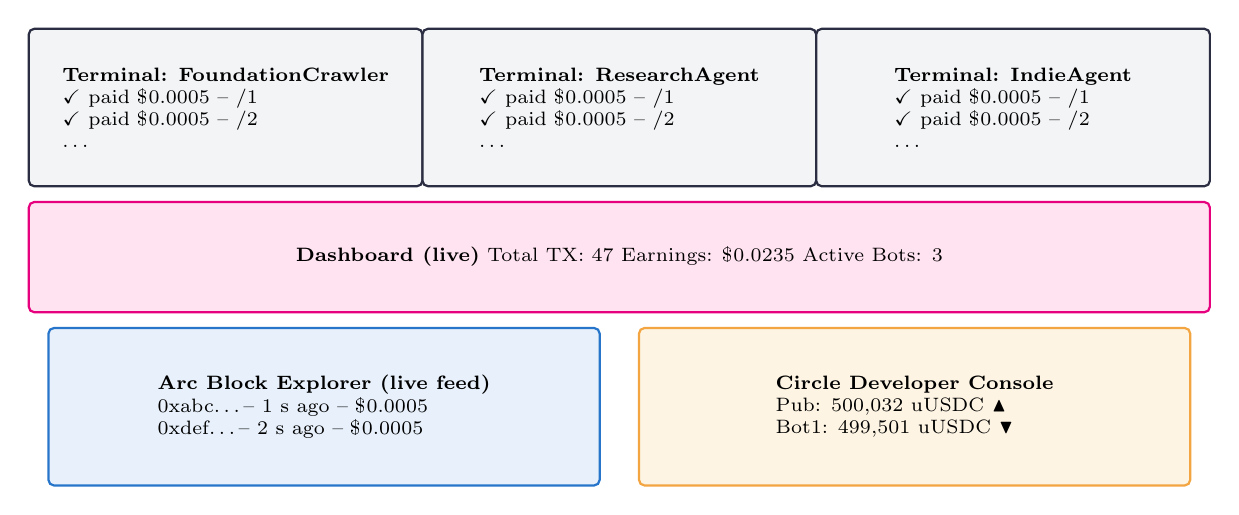
\begin{tikzpicture}[
  frame/.style={draw, thick, rounded corners=2pt, minimum width=5cm, minimum height=2cm, align=left, font=\scriptsize, inner sep=2mm}
]
\node[frame, fill=tollgategraylight, draw=tollgateslate] (f1) at (-5,4) {\textbf{Terminal: FoundationCrawler}\\ $\checkmark$ paid \$0.0005 -- /1\\ $\checkmark$ paid \$0.0005 -- /2\\ \ldots};
\node[frame, fill=tollgategraylight, draw=tollgateslate] (f2) at (0,4) {\textbf{Terminal: ResearchAgent}\\ $\checkmark$ paid \$0.0005 -- /1\\ $\checkmark$ paid \$0.0005 -- /2\\ \ldots};
\node[frame, fill=tollgategraylight, draw=tollgateslate] (f3) at (5,4) {\textbf{Terminal: IndieAgent}\\ $\checkmark$ paid \$0.0005 -- /1\\ $\checkmark$ paid \$0.0005 -- /2\\ \ldots};

\node[frame, fill=tollgatepinklight, draw=tollgatepink, minimum width=15cm, minimum height=1.4cm] (dash) at (0,2.1) {\textbf{Dashboard (live)} \hfill Total TX: 47 \hfill Earnings: \$0.0235 \hfill Active Bots: 3};

\node[frame, fill=tollgatearclight, draw=tollgatearc, minimum width=7cm] (ex) at (-3.75,0.2) {\textbf{Arc Block Explorer (live feed)}\\ 0xabc\ldots -- 1 s ago -- \$0.0005\\ 0xdef\ldots -- 2 s ago -- \$0.0005};
\node[frame, fill=tollgategoldlight, draw=tollgategold, minimum width=7cm] (cc) at (3.75,0.2) {\textbf{Circle Developer Console}\\ Pub: 500,032 uUSDC $\blacktriangle$\\ Bot1: 499,501 uUSDC $\blacktriangledown$};
\end{tikzpicture}
\end{center}

\subsection{Margin Reveal}

\begin{table}[H]
\centering
\footnotesize
\begin{tabularx}{\textwidth}{@{} l R{2.5cm} R{2.5cm} R{2.5cm} @{}}
\toprule
\textbf{Metric (60 TX)} & \textbf{Arc} & \textbf{Ethereum} & \textbf{Polygon} \\
\midrule
Revenue & \$0.0300 & \$0.0300 & \$0.0300 \\
Gas spent & \$0.00120 & \$30.00 & \$0.60 \\
Net profit & \$0.02880 & -\$29.97 & -\$0.57 \\
Margin \% & \textbf{96\%} & \textbf{-99,900\%} & \textbf{-1,900\%} \\
\bottomrule
\end{tabularx}
\end{table}

\begin{highlightbox}[title={\iconCheck~ Why Arc wins this math}]
Arc denominates gas in USDC. Gas cost is fixed at design time, not probabilistic at runtime. Ethereum's native-token gas spikes turn any sub-cent business into a loss on any request. Arc is the only chain where this model is mathematically profitable.
\end{highlightbox}

\newpage

%===============================================================================
% SECTION 10: BUILD PLAN
%===============================================================================
\section{Five-Day Build Plan}

\begin{table}[H]
\centering
\footnotesize
\begin{tabularx}{\textwidth}{@{} l l X @{}}
\toprule
\textbf{Day} & \textbf{Focus} & \textbf{Deliverables} \\
\midrule
1 & Foundations & Arc RPC wired, USDC contract referenced, Circle Developer account active, testnet faucet drained into four wallets, first hello-world TX visible on Arc Explorer. \\
2 & Core middleware & Express + Hono + Cloudflare Worker middleware with 402 response shape, x402 integration, HMAC receipt signer, publisher dashboard scaffold. \\
3 & Agent flow & Agent SDK (Node) auto-handles 402, signs via Circle Wallets, retries with proof. AIsa API integration. Circle Gateway multi-chain balance. \\
4 & Reputation + off-ramp & ERC-8004-vyper contract deployed via Circle-titanoboa SDK. Publisher withdraw flow using CCTP. Dashboard live counters via Convex subscriptions. \\
5 & Polish + submission & Record demo through Circle Developer Console and Arc Explorer. Write 1,500-word Product Feedback. Push repo public. Submit. \\
\bottomrule
\end{tabularx}
\end{table}

\subsection{Risk Tiering}

\begin{table}[H]
\centering
\footnotesize
\begin{tabularx}{\textwidth}{@{} l X @{}}
\toprule
\textbf{Tier} & \textbf{What ships} \\
\midrule
Tier 1 (must ship) & Arc, USDC, Nanopayments, Circle Wallets, x402, Arc Explorer, Circle Console. Without these there is no submission. \\
Tier 2 (ship if Day 1-3 on track) & AIsa integration, Circle Gateway, ERC-8004-vyper. These turn a viable submission into a winning one. \\
Tier 3 (document if time runs out) & Bridge Kit full flow, Vyper contract suite, self-hosted facilitator. Slide only if not shippable. \\
\bottomrule
\end{tabularx}
\end{table}

\newpage

%===============================================================================
% SECTION 11: PRODUCT INVENTORY
%===============================================================================
\section{Product Inventory}

\begin{table}[H]
\centering
\footnotesize
\begin{tabularx}{\textwidth}{@{} c l l l X @{}}
\toprule
\textbf{\#} & \textbf{Product} & \textbf{MVP?} & \textbf{Who pays} & \textbf{Revenue model} \\
\midrule
1 & Middleware SDK & Yes & Publisher dev & Free, open source \\
2 & Agent SDK & Yes & Agent dev & Free, open source \\
3 & Dashboard & Yes & Publisher & Free tier + Pro \$29/mo \\
4 & Hosted Gateway & Year 1 & Non-technical pub & 5\% of earnings \\
5 & Facilitator & Year 1 & Infra / enterprise & Per-verify fee \\
6 & Reputation Oracle & Year 1 & Agent + publisher & Free read, stake to write \\
7 & Explorer & Year 2 & Public & Premium search \\
8 & Analytics API & Year 2 & Enterprise publisher & Usage-based \\
9 & WAF Integrations & Year 2 & Enterprise & Included Pro+ \\
10 & Platform Plugins (WordPress, Ghost, Shopify) & Year 2 & Long-tail publisher & Included \\
\bottomrule
\end{tabularx}
\end{table}

\subsection{Three-Leg Tripod}

\begin{highlightbox}[title={\iconCheck~ What we build in five days}]
\textbf{Middleware SDK} collects payments. \textbf{Agent SDK} sends payments. \textbf{Dashboard} proves the flow.

That is the tripod. Products 4 through 10 are commercialization and scale, worth sketching on the roadmap slide but not worth building for the demo.
\end{highlightbox}

\newpage

%===============================================================================
% SECTION 12: ICP
%===============================================================================
\section{Ideal Customer Profiles}

\subsection{Six Profiles, Two Sides}

\begin{table}[H]
\centering
\footnotesize
\begin{tabularx}{\textwidth}{@{} c l l l l X @{}}
\toprule
\textbf{\#} & \textbf{Profile} & \textbf{Side} & \textbf{Priority} & \textbf{Deal size} & \textbf{Adoption speed} \\
\midrule
P1 & Technical content publisher (docs, dev blogs) & Earn & High & Self-serve \$0-\$199/mo & Days \\
P2 & Trade / niche media with dev resources & Earn & High & Pro \$199-\$999/mo & Weeks \\
P3 & Mid-tier AI company positioning on ethics & Pay & High & Free SDK + facilitator fee & Days \\
E1 & Enterprise media conglomerate & Earn & Expansion & \$5K-\$25K/mo & 6-12 months \\
E2 & Enterprise internal AI team (Fortune 500) & Pay & Expansion & \$50K-\$500K/yr & 6-9 months \\
E3 & AI research institution (academic) & Pay & Expansion & Free + fee & 1-3 months \\
\bottomrule
\end{tabularx}
\end{table}

\subsection{Beachhead}

\begin{archbox}[title={\iconGate~ Week-1 target after launch}]
\textbf{P1: Technical Content Publishers.} Docs sites, dev blogs, technical Substacks, engineering community sites. Dev teams install SDKs same-day. Crypto-native, no USDC education needed. Public community distribution (HackerNews, X) is free. Fifty P1 wins become the case-study base that later unlocks P2 trade media and E1 enterprise.
\end{archbox}

\newpage

%===============================================================================
% SECTION 13: CLAUDE CODE BUILD ORCHESTRATION
%===============================================================================
\section{Claude Code Build Orchestration}

\begin{tollbox}[title={\iconCog~ Who codes Tollgate}]
Tollgate is built by an orchestrated team of Claude Code agents, each specialized for a discrete part of the stack. Twelve agents in total: eight general-purpose agents from the knowledge brain and four Tollgate-specific agents that handle blockchain, Circle, x402, and demo orchestration.

Each agent reads its \texttt{AGENT.md} (process + checklist) before running, produces a report in its \texttt{REPORT-TEMPLATE.md} format, and hands off to the next agent in the chain. Nothing is improvised. Every phase has an owner.
\end{tollbox}

\subsection{Agent Roster}

\begin{table}[H]
\centering
\footnotesize
\begin{tabularx}{\textwidth}{@{} l l X @{}}
\toprule
\textbf{\#} & \textbf{Agent} & \textbf{Responsibility in Tollgate build} \\
\midrule
\multicolumn{3}{@{}l}{\textit{General-purpose agents (from Claude knowledge brain)}} \\
\midrule
1 & tech-stack-detector & Confirm Node 20, TypeScript, Next.js 16, Convex, Clerk, Cloudflare Workers, Vyper. Flag drift. \\
2 & code-analyzer & Map repo structure at every checkpoint. Produce module-level summary. \\
3 & architecture-mapper & Keep this architecture document in sync with code. Detect diverged diagrams. \\
4 & code-auditor & Review every PR against naming, structure, anti-patterns, correctness, maintainability. \\
5 & security-scanner & Scan 402 flow, HMAC receipts, nonce replay, Circle key storage, Clerk JWT handling, CORS. \\
6 & performance-profiler & Measure hot paths: cached request p95 $<$ 50 ms, cold p95 $<$ 1.2 s, edge KV lookup. \\
7 & dependency-auditor & Audit Circle SDK, Convex SDK, x402 client, ERC-8004 ABI, OpenRouter (if used). \\
8 & documentation-generator & Produce README, SDK docs, install guide, Circle Product Feedback write-up. \\
\midrule
\multicolumn{3}{@{}l}{\textit{Tollgate-specific agents (built for this project)}} \\
\midrule
9 & arc-chain-agent & Arc RPC client, TX signing, contract deployment via Circle-titanoboa, event parsing. \\
10 & circle-integration-agent & Circle Wallets provisioning, Gateway balance queries, CCTP bridge calls, webhook HMAC verify. \\
11 & x402-protocol-agent & 402 response builder, facilitator client, nonce generator, receipt HMAC signer and verifier. \\
12 & demo-orchestrator-agent & Fund 3 testnet wallets, launch parallel scrapers, capture TX hashes, produce Arc Explorer bookmarks. \\
\bottomrule
\end{tabularx}
\end{table}

\subsection{Orchestration Diagram}

\begin{center}
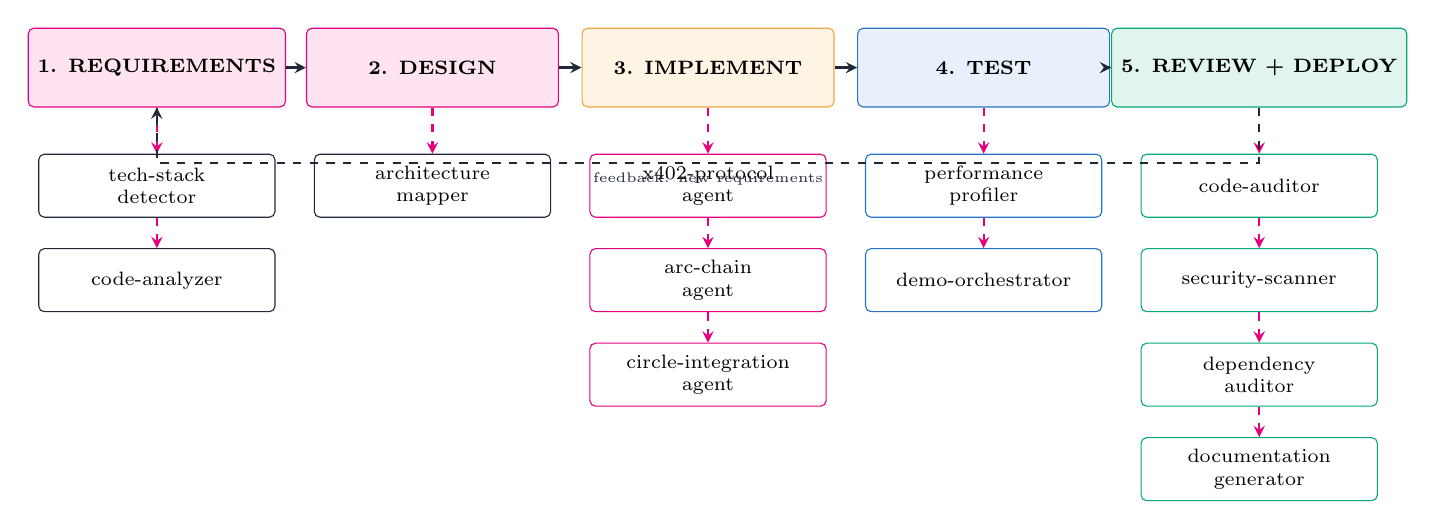
\begin{tikzpicture}[
  x=1cm, y=1cm,
  phase/.style={draw, rounded corners=2pt, minimum width=3.2cm, minimum height=1.0cm, align=center, font=\scriptsize\bfseries, inner sep=1.2mm},
  agent/.style={draw, rounded corners=2pt, minimum width=3.0cm, minimum height=0.8cm, align=center, font=\scriptsize, inner sep=1mm},
  flow/.style={-stealth, thick, tollgatecharcoal},
  side/.style={-stealth, thick, tollgatepink, dashed}
]

% Phases (top row)
\node[phase, fill=tollgatepinklight, draw=tollgatepink] (p1) at (-6,6) {1. REQUIREMENTS};
\node[phase, fill=tollgatepinklight, draw=tollgatepink] (p2) at (-2.5,6) {2. DESIGN};
\node[phase, fill=tollgategoldlight, draw=tollgategold] (p3) at (1,6) {3. IMPLEMENT};
\node[phase, fill=tollgatearclight, draw=tollgatearc] (p4) at (4.5,6) {4. TEST};
\node[phase, fill=tollgategreenlight, draw=tollgategreen] (p5) at (8,6) {5. REVIEW + DEPLOY};

\draw[flow] (p1) -- (p2);
\draw[flow] (p2) -- (p3);
\draw[flow] (p3) -- (p4);
\draw[flow] (p4) -- (p5);

% Agents by phase (columns below each phase)
\node[agent, fill=white, draw=tollgatecharcoal] (a1a) at (-6,4.5) {tech-stack\\ detector};
\node[agent, fill=white, draw=tollgatecharcoal] (a1b) at (-6,3.3) {code-analyzer};

\node[agent, fill=white, draw=tollgatecharcoal] (a2a) at (-2.5,4.5) {architecture\\ mapper};

\node[agent, fill=white, draw=tollgatepink] (a3a) at (1,4.5) {x402-protocol\\ agent};
\node[agent, fill=white, draw=tollgatepink] (a3b) at (1,3.3) {arc-chain\\ agent};
\node[agent, fill=white, draw=tollgatepink] (a3c) at (1,2.1) {circle-integration\\ agent};

\node[agent, fill=white, draw=tollgatearc] (a4a) at (4.5,4.5) {performance\\ profiler};
\node[agent, fill=white, draw=tollgatearc] (a4b) at (4.5,3.3) {demo-orchestrator};

\node[agent, fill=white, draw=tollgategreen] (a5a) at (8,4.5) {code-auditor};
\node[agent, fill=white, draw=tollgategreen] (a5b) at (8,3.3) {security-scanner};
\node[agent, fill=white, draw=tollgategreen] (a5c) at (8,2.1) {dependency\\ auditor};
\node[agent, fill=white, draw=tollgategreen] (a5d) at (8,0.9) {documentation\\ generator};

% Phase-to-agent links
\draw[side] (p1) -- (a1a);
\draw[side] (a1a) -- (a1b);
\draw[side] (p2) -- (a2a);
\draw[side] (p3) -- (a3a);
\draw[side] (a3a) -- (a3b);
\draw[side] (a3b) -- (a3c);
\draw[side] (p4) -- (a4a);
\draw[side] (a4a) -- (a4b);
\draw[side] (p5) -- (a5a);
\draw[side] (a5a) -- (a5b);
\draw[side] (a5b) -- (a5c);
\draw[side] (a5c) -- (a5d);

% Feedback loop
\draw[flow, dashed] (p5.south) -- ++(0,-0.7) -| node[pos=0.25, below, font=\tiny] {feedback: new requirements} (p1.south);

\end{tikzpicture}
\end{center}

\subsection{Build Phases Mapped to Agents}

\begin{table}[H]
\centering
\footnotesize
\begin{tabularx}{\textwidth}{@{} l X X @{}}
\toprule
\textbf{Phase} & \textbf{Primary agents} & \textbf{Deliverable} \\
\midrule
1. Requirements & tech-stack-detector, code-analyzer & Stack confirmation report, repo baseline map. \\
2. Design & architecture-mapper & This document, kept current. \\
3. Implement & x402-protocol-agent, arc-chain-agent, circle-integration-agent & Working middleware, agent SDK, dashboard. \\
4. Test & performance-profiler, demo-orchestrator-agent & p95 benchmarks; 60-TX demo running on testnet. \\
5. Review & code-auditor, security-scanner, dependency-auditor & PR-by-PR audit reports. No merge without green checks. \\
6. Deploy & CI / CD pipeline (GitHub Actions) & Vercel preview per PR, Convex deploy on main. \\
7. Monitor & Sentry, Axiom, Convex dashboard, PostHog & Live alerting; feedback into next requirements cycle. \\
\bottomrule
\end{tabularx}
\end{table}

\subsection{Agent Handoff Rules}

\begin{flowbox}[title={\iconCheck~ How agents pass work to each other}]
\begin{itemize}[leftmargin=*]
  \item \textbf{Read before act.} Every agent reads its \texttt{AGENT.md} before starting. Output uses the \texttt{REPORT-TEMPLATE.md} format.
  \item \textbf{One source of truth per concern.} Only arc-chain-agent touches Arc RPC. Only circle-integration-agent touches Circle APIs. Only x402-protocol-agent touches 402 and receipt formats. Prevents duplicate or conflicting client code.
  \item \textbf{No merge without audit.} code-auditor, security-scanner, and dependency-auditor must all pass on every PR before merge. No exceptions for demo pressure.
  \item \textbf{Performance gates are code gates.} performance-profiler runs on every PR that touches middleware or facilitator. A regression blocks merge.
  \item \textbf{Demo orchestrator owns the demo.} Day 5 video recording is its job. No code changes accepted on Day 5 except from demo-orchestrator.
  \item \textbf{Feedback loop.} After deploy, monitoring reports feed into new requirement tickets, not ad-hoc bug fixes. Coherence over speed.
\end{itemize}
\end{flowbox}

\subsection{Why This Matters for the Hackathon}

\begin{archbox}[title={\iconStar~ Agent orchestration is a judge-signal}]
Most solo hackers hand-roll everything. Tollgate demonstrates a disciplined, agent-orchestrated build that produces an auditable trail: every PR reviewed by named agents, every integration owned by a specialist, every benchmark enforced automatically. Judges who open the repo see structure, not scaffolding.

This matters because the hackathon brief explicitly rewards production-readiness. The agents are not cosmetic. They enforce the non-functional requirements that this architecture document commits to.
\end{archbox}

\newpage

%===============================================================================
% APPENDIX A: TECH STACK
%===============================================================================
\section*{Appendix A: Tech Stack Summary}
\addcontentsline{toc}{section}{Appendix A: Tech Stack Summary}

\begin{table}[H]
\centering
\footnotesize
\begin{tabularx}{\textwidth}{@{} l X @{}}
\toprule
\textbf{Layer} & \textbf{Chosen tech} \\
\midrule
Frontend (dashboard) & Next.js 16 (App Router, React 19), Tailwind 4, Shadcn/ui \\
Frontend (marketing) & Same repo, static pre-render \\
Auth & Clerk (@clerk/nextjs), JWT template \texttt{convex} \\
Backend & Convex (queries, mutations, actions, scheduler, search, vector, R2 storage bridge) \\
Edge runtime & Cloudflare Workers (hosted gateway + telemetry) \\
Middleware libs & @tollgate/express, @tollgate/hono, @tollgate/cloudflare-worker \\
Agent libs & @tollgate/agent (Node), tollgate-agent (Python) \\
Payments & USDC on Arc via Circle Nanopayments + x402 \\
Wallets & Circle Wallets (publisher custody), self-custody optional (agents) \\
Cross-chain & Circle Gateway (balance), Bridge Kit / CCTP (off-ramp) \\
Smart contracts & ERC-8004-vyper (reputation), USDC (Circle deployment) \\
Vyper tooling & Circle-titanoboa-sdk for local simulation \\
Data upstream & AIsa Nanopayment APIs \\
Observability & Sentry (errors), Axiom (logs), PostHog (product), Convex dashboard \\
CI/CD & GitHub Actions $\rightarrow$ Vercel preview on PR, Convex deploy on merge to main \\
Domains & tollgate.brianmwai.com (dashboard), demo-news.brianmwai.com (demo site), api.tollgate.brianmwai.com (gateway) \\
\bottomrule
\end{tabularx}
\end{table}

%===============================================================================
% APPENDIX B: GLOSSARY
%===============================================================================
\section*{Appendix B: Glossary}
\addcontentsline{toc}{section}{Appendix B: Glossary}

\begin{table}[H]
\centering
\footnotesize
\begin{tabularx}{\textwidth}{@{} l X @{}}
\toprule
\textbf{Term} & \textbf{Definition} \\
\midrule
402 & HTTP status code \texttt{Payment Required}, reserved since RFC 2616 (1997), activated for programmatic use by x402. \\
Arc & Circle's purpose-built Layer-1 blockchain for stablecoin settlement. USDC is the native gas token. \\
CCTP & Cross-Chain Transfer Protocol, Circle's native bridging of USDC across supported chains. \\
Circle Gateway & Unified USDC balance view across chains. Enables single-balance spending. \\
Circle Wallets & Circle's programmable wallet API, custodial or smart wallet flavors. \\
ERC-8004 & Emerging standard for onchain agent identity, reputation, and validation. \\
Facilitator & Service that verifies x402 payment proofs against the chain before content is served. \\
Nanopayments & Circle's primitive for high-frequency, sub-cent transactions with deterministic fees. \\
Nonce & Single-use identifier in the 402 response that prevents replay attacks. \\
Receipt & HMAC-signed short-TTL token that lets an agent skip onchain verification on repeat requests. \\
uUSDC & Micro-USDC, equal to 10$^{-6}$ USDC. Unit in which Tollgate prices are stored. \\
Vyper & Python-flavored smart-contract language, used for ERC-8004 implementation. \\
x402 & Open web payment standard built on HTTP 402, with facilitator-verified proofs. \\
\bottomrule
\end{tabularx}
\end{table}

%===============================================================================
% APPENDIX C: REFERENCES
%===============================================================================
\section*{Appendix C: References}
\addcontentsline{toc}{section}{Appendix C: References}

\begin{itemize}[leftmargin=*]
  \item Arc Documentation -- \href{https://arc.network/docs}{arc.network/docs}
  \item Circle Developer Docs -- \href{https://developers.circle.com}{developers.circle.com}
  \item Circle Nanopayments -- \href{https://developers.circle.com/nanopayments}{developers.circle.com/nanopayments}
  \item x402 Specification -- \href{https://x402.org}{x402.org}
  \item ERC-8004 Draft -- \href{https://eips.ethereum.org/EIPS/eip-8004}{EIP-8004}
  \item Circle Github -- \href{https://github.com/circlefin}{github.com/circlefin}
  \item AIsa API Collection -- \href{https://github.com/aisa-xyz}{github.com/aisa-xyz}
  \item Tollgate Repository -- \href{https://github.com/brn-mwai/tollgate}{github.com/brn-mwai/tollgate}
\end{itemize}

\newpage

%===============================================================================
% APPENDIX D: REFERENCE DIAGRAMS FROM KNOWLEDGE BRAIN
%===============================================================================
\section*{Appendix D: Reference Diagrams from Knowledge Brain}
\addcontentsline{toc}{section}{Appendix D: Reference Diagrams from Knowledge Brain}

\begin{archbox}[title={\iconCog~ Provenance}]
The following diagrams come from the engineering knowledge base at \texttt{Claude\_brain/diagrams/}. Each is a general-purpose pattern applied here to Tollgate. Keeping them in this document means the build team can see both the abstract pattern and the Tollgate instantiation side by side.
\end{archbox}

\subsection*{D.1 Seven-Step System Design Framework}

\begin{center}
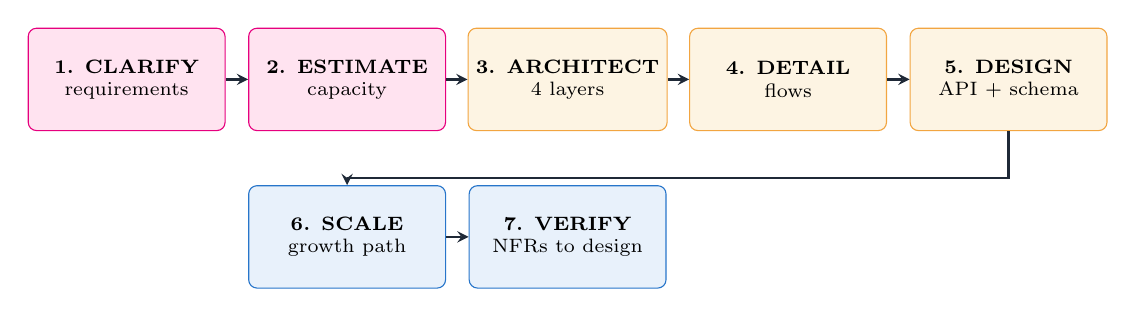
\begin{tikzpicture}[
  x=1cm, y=1cm,
  stp/.style={draw, rounded corners=3pt, minimum width=2.5cm, minimum height=1.3cm, align=center, font=\scriptsize\bfseries, inner sep=1mm},
  arr/.style={-stealth, thick, tollgatecharcoal}
]
\node[stp, fill=tollgatepinklight, draw=tollgatepink] (s1) at (0,0) {1. CLARIFY\\ \normalfont\scriptsize requirements};
\node[stp, fill=tollgatepinklight, draw=tollgatepink] (s2) at (2.8,0) {2. ESTIMATE\\ \normalfont\scriptsize capacity};
\node[stp, fill=tollgategoldlight, draw=tollgategold] (s3) at (5.6,0) {3. ARCHITECT\\ \normalfont\scriptsize 4 layers};
\node[stp, fill=tollgategoldlight, draw=tollgategold] (s4) at (8.4,0) {4. DETAIL\\ \normalfont\scriptsize flows};
\node[stp, fill=tollgategoldlight, draw=tollgategold] (s5) at (11.2,0) {5. DESIGN\\ \normalfont\scriptsize API + schema};
\node[stp, fill=tollgatearclight, draw=tollgatearc] (s6) at (2.8,-2) {6. SCALE\\ \normalfont\scriptsize growth path};
\node[stp, fill=tollgatearclight, draw=tollgatearc] (s7) at (5.6,-2) {7. VERIFY\\ \normalfont\scriptsize NFRs to design};

\draw[arr] (s1) -- (s2);
\draw[arr] (s2) -- (s3);
\draw[arr] (s3) -- (s4);
\draw[arr] (s4) -- (s5);
\draw[arr] (s5.south) -- ++(0,-0.6) -| (s6.north);
\draw[arr] (s6) -- (s7);
\end{tikzpicture}
\end{center}

\textit{Applied: Sections 1 through 7 of this document.}

\subsection*{D.2 Coding System Seven-Phase Process}

\begin{center}
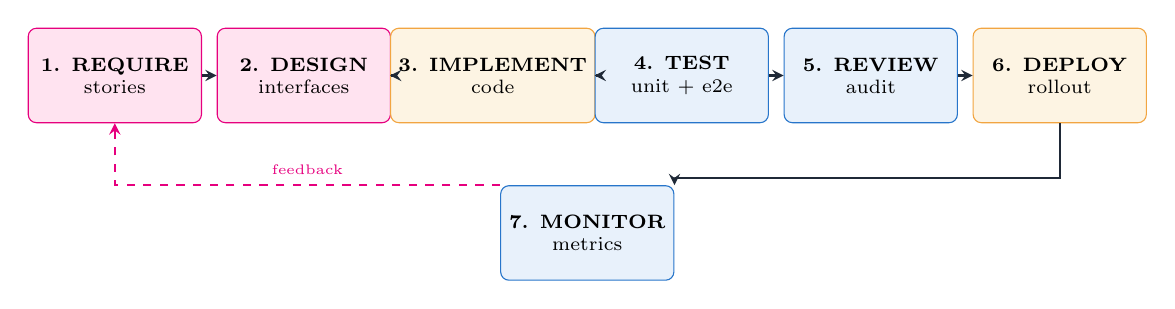
\begin{tikzpicture}[
  x=1cm, y=1cm,
  ph/.style={draw, rounded corners=3pt, minimum width=2.2cm, minimum height=1.2cm, align=center, font=\scriptsize\bfseries, inner sep=1mm},
  arr/.style={-stealth, thick, tollgatecharcoal},
  fb/.style={-stealth, dashed, thick, tollgatepink}
]
\node[ph, fill=tollgatepinklight, draw=tollgatepink] (q1) at (0,0) {1. REQUIRE\\ \normalfont\scriptsize stories};
\node[ph, fill=tollgatepinklight, draw=tollgatepink] (q2) at (2.4,0) {2. DESIGN\\ \normalfont\scriptsize interfaces};
\node[ph, fill=tollgategoldlight, draw=tollgategold] (q3) at (4.8,0) {3. IMPLEMENT\\ \normalfont\scriptsize code};
\node[ph, fill=tollgatearclight, draw=tollgatearc] (q4) at (7.2,0) {4. TEST\\ \normalfont\scriptsize unit + e2e};
\node[ph, fill=tollgatearclight, draw=tollgatearc] (q5) at (9.6,0) {5. REVIEW\\ \normalfont\scriptsize audit};
\node[ph, fill=tollgategoldlight, draw=tollgategold] (q6) at (12.0,0) {6. DEPLOY\\ \normalfont\scriptsize rollout};
\node[ph, fill=tollgatearclight, draw=tollgatearc] (q7) at (6.0,-2) {7. MONITOR\\ \normalfont\scriptsize metrics};

\draw[arr] (q1) -- (q2);
\draw[arr] (q2) -- (q3);
\draw[arr] (q3) -- (q4);
\draw[arr] (q4) -- (q5);
\draw[arr] (q5) -- (q6);
\draw[arr] (q6.south) -- ++(0,-0.7) -| (q7.north east);
\draw[fb] (q7.north west) -| node[pos=0.25, above, font=\tiny] {feedback} (q1.south);
\end{tikzpicture}
\end{center}

\textit{Applied: Section 13 Claude Code Build Orchestration.}

\subsection*{D.3 Payment Flow with Idempotency and Outbox}

Tollgate reuses the Stripe-style payment pattern: idempotency keys prevent double-charge, and a transactional outbox prevents event-DB divergence.

\begin{center}
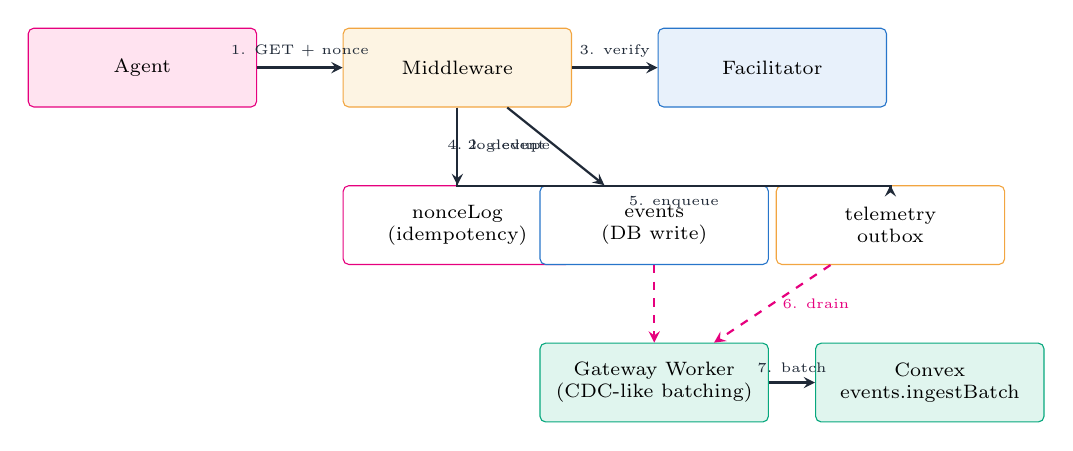
\begin{tikzpicture}[
  x=1cm, y=1cm,
  box/.style={draw, rounded corners=2pt, minimum width=2.9cm, minimum height=1.0cm, align=center, font=\scriptsize, inner sep=1mm},
  db/.style={draw, cylinder, shape border rotate=90, aspect=0.2, minimum width=2.4cm, minimum height=1.2cm, align=center, font=\scriptsize, inner sep=1mm},
  arr/.style={-stealth, thick, tollgatecharcoal},
  dot/.style={-stealth, dashed, tollgatepink, thick}
]
\node[box, fill=tollgatepinklight, draw=tollgatepink] (agent) at (-5,4) {Agent};
\node[box, fill=tollgategoldlight, draw=tollgategold] (mw) at (-1,4) {Middleware};
\node[box, fill=tollgatearclight, draw=tollgatearc] (fac) at (3,4) {Facilitator};

\node[box, fill=white, draw=tollgatepink] (nonce) at (-1,2) {nonceLog\\ (idempotency)};
\node[box, fill=white, draw=tollgatearc] (events) at (1.5,2) {events\\ (DB write)};
\node[box, fill=white, draw=tollgategold] (outbox) at (4.5,2) {telemetry\\ outbox};

\node[box, fill=tollgategreenlight, draw=tollgategreen] (worker) at (1.5,0) {Gateway Worker\\ (CDC-like batching)};
\node[box, fill=tollgategreenlight, draw=tollgategreen] (convex) at (5,0) {Convex\\ events.ingestBatch};

\draw[arr] (agent) -- node[above, font=\tiny] {1. GET + nonce} (mw);
\draw[arr] (mw) -- node[right, font=\tiny] {2. dedupe} (nonce);
\draw[arr] (mw) -- node[above, font=\tiny] {3. verify} (fac);
\draw[arr] (mw) -- node[font=\tiny, left] {4. log event} (events);
\draw[arr] (mw.south) -- ++(0,-1) -| node[pos=0.25, below, font=\tiny] {5. enqueue} (outbox.north);
\draw[dot] (outbox) -- node[right, font=\tiny] {6. drain} (worker);
\draw[dot] (events) -- node[left, font=\tiny] {} (worker);
\draw[arr] (worker) -- node[above, font=\tiny] {7. batch} (convex);
\end{tikzpicture}
\end{center}

\textit{Applied: nonceLog table plus edge telemetry outbox plus Convex batching in Section 5.}

\subsection*{D.4 Caching Strategy Layers}

Each layer sits closer to the agent than the next. A cache hit at any layer skips everything below.

\begin{center}
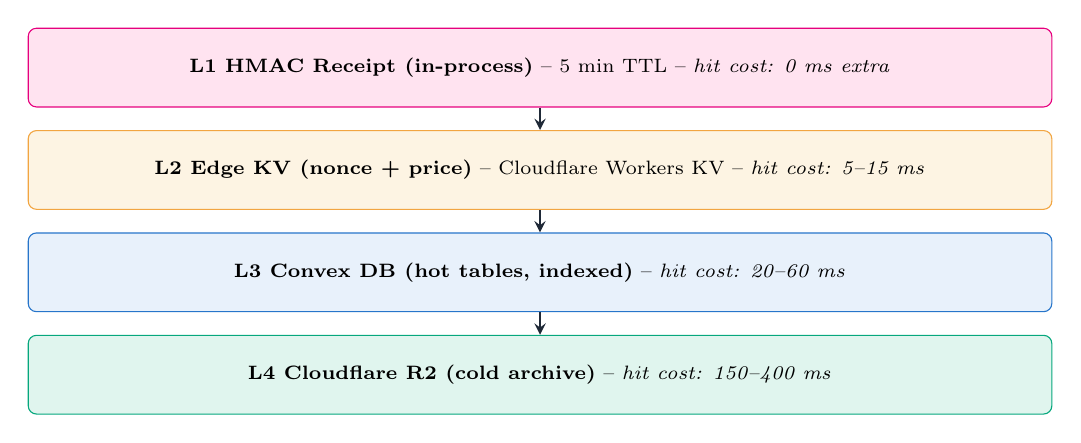
\begin{tikzpicture}[
  x=1cm, y=1cm,
  layer/.style={draw, rounded corners=3pt, minimum width=13cm, minimum height=1.0cm, align=left, font=\scriptsize, inner sep=2mm},
  arr/.style={-stealth, thick, tollgatecharcoal}
]
\node[layer, fill=tollgatepinklight, draw=tollgatepink] (l1) at (0,4) {\textbf{L1 HMAC Receipt (in-process)} -- 5 min TTL -- \textit{hit cost: 0 ms extra}};
\node[layer, fill=tollgategoldlight, draw=tollgategold] (l2) at (0,2.7) {\textbf{L2 Edge KV (nonce + price)} -- Cloudflare Workers KV -- \textit{hit cost: 5--15 ms}};
\node[layer, fill=tollgatearclight, draw=tollgatearc] (l3) at (0,1.4) {\textbf{L3 Convex DB (hot tables, indexed)} -- \textit{hit cost: 20--60 ms}};
\node[layer, fill=tollgategreenlight, draw=tollgategreen] (l4) at (0,0.1) {\textbf{L4 Cloudflare R2 (cold archive)} -- \textit{hit cost: 150--400 ms}};

\draw[arr] (l1) -- (l2);
\draw[arr] (l2) -- (l3);
\draw[arr] (l3) -- (l4);
\end{tikzpicture}
\end{center}

\textit{Applied: the receipt collapses 50 requests into 1 onchain TX. Cache invalidation is TTL-only, matching the brain guidance that short TTLs beat complex invalidation.}

\subsection*{D.5 Message Queue Pattern (Telemetry Outbox)}

\begin{center}
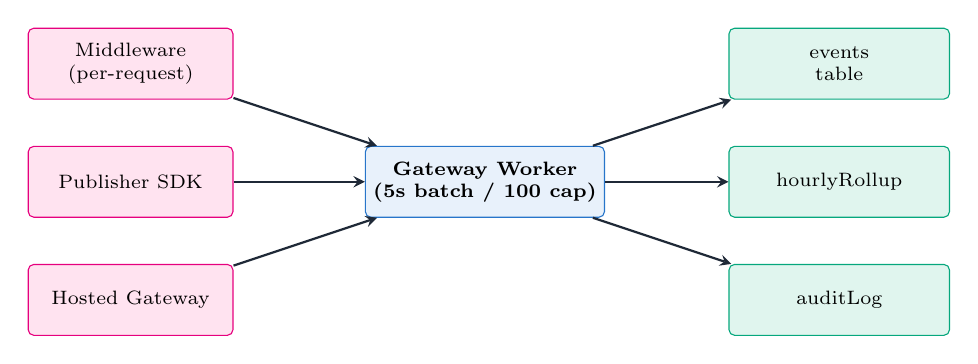
\begin{tikzpicture}[
  x=1cm, y=1cm,
  src/.style={draw, rounded corners=2pt, minimum width=2.6cm, minimum height=0.9cm, align=center, font=\scriptsize, inner sep=1mm},
  mq/.style={draw, rounded corners=2pt, minimum width=3.0cm, minimum height=0.9cm, align=center, font=\scriptsize\bfseries, inner sep=1mm, fill=tollgatearclight},
  cons/.style={draw, rounded corners=2pt, minimum width=2.8cm, minimum height=0.9cm, align=center, font=\scriptsize, inner sep=1mm},
  arr/.style={-stealth, thick, tollgatecharcoal}
]
\node[src, fill=tollgatepinklight, draw=tollgatepink] (p1) at (-5.5,2) {Middleware\\ (per-request)};
\node[src, fill=tollgatepinklight, draw=tollgatepink] (p2) at (-5.5,0.5) {Publisher SDK};
\node[src, fill=tollgatepinklight, draw=tollgatepink] (p3) at (-5.5,-1) {Hosted Gateway};

\node[mq, draw=tollgatearc] (q) at (-1,0.5) {Gateway Worker\\ (5s batch / 100 cap)};

\node[cons, fill=tollgategreenlight, draw=tollgategreen] (c1) at (3.5,2) {events\\ table};
\node[cons, fill=tollgategreenlight, draw=tollgategreen] (c2) at (3.5,0.5) {hourlyRollup};
\node[cons, fill=tollgategreenlight, draw=tollgategreen] (c3) at (3.5,-1) {auditLog};

\draw[arr] (p1) -- (q);
\draw[arr] (p2) -- (q);
\draw[arr] (p3) -- (q);
\draw[arr] (q) -- (c1);
\draw[arr] (q) -- (c2);
\draw[arr] (q) -- (c3);
\end{tikzpicture}
\end{center}

\textit{Applied: fanout pattern plus outbox means new consumers (audit, analytics, compliance export) can subscribe without touching publisher code.}

\subsection*{D.6 Database Decision That Led to Convex}

\begin{center}
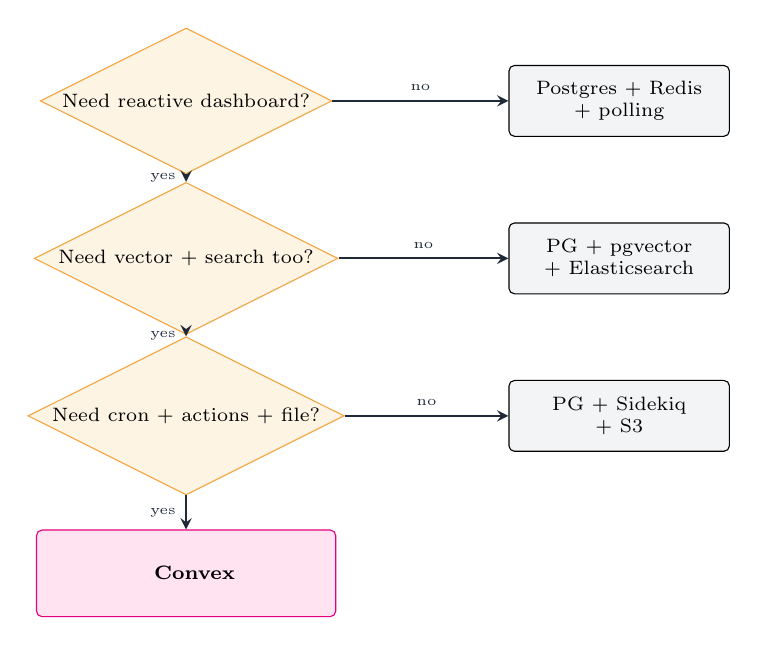
\begin{tikzpicture}[
  x=1cm, y=1cm,
  q/.style={draw, diamond, aspect=2, minimum width=3.5cm, minimum height=0.5cm, align=center, font=\scriptsize, inner sep=1pt, fill=tollgategoldlight, draw=tollgategold},
  opt/.style={draw, rounded corners=2pt, minimum width=2.8cm, minimum height=0.9cm, align=center, font=\scriptsize, inner sep=1mm},
  result/.style={draw, rounded corners=2pt, minimum width=3.8cm, minimum height=1.1cm, align=center, font=\scriptsize\bfseries, inner sep=1mm, fill=tollgatepinklight, draw=tollgatepink},
  arr/.style={-stealth, thick, tollgatecharcoal}
]
\node[q] (q1) at (0,6) {Need reactive dashboard?};
\node[opt, fill=tollgategraylight] (skip) at (5.5,6) {Postgres + Redis\\ + polling};
\node[q] (q2) at (0,4) {Need vector + search too?};
\node[opt, fill=tollgategraylight] (sep) at (5.5,4) {PG + pgvector\\ + Elasticsearch};
\node[q] (q3) at (0,2) {Need cron + actions + file?};
\node[opt, fill=tollgategraylight] (stack) at (5.5,2) {PG + Sidekiq\\ + S3};
\node[result] (res) at (0,0) {\iconCheck~ Convex};

\draw[arr] (q1) -- node[above, font=\tiny] {no} (skip);
\draw[arr] (q1) -- node[left, font=\tiny] {yes} (q2);
\draw[arr] (q2) -- node[above, font=\tiny] {no} (sep);
\draw[arr] (q2) -- node[left, font=\tiny] {yes} (q3);
\draw[arr] (q3) -- node[above, font=\tiny] {no} (stack);
\draw[arr] (q3) -- node[left, font=\tiny] {yes} (res);
\end{tikzpicture}
\end{center}

\textit{Applied: Tollgate hits yes on all three gates (reactive dashboard, vector + search for agent clustering, cron plus actions plus file storage). Convex replaces four systems with one.}

\newpage

\vspace{1cm}

\begin{center}
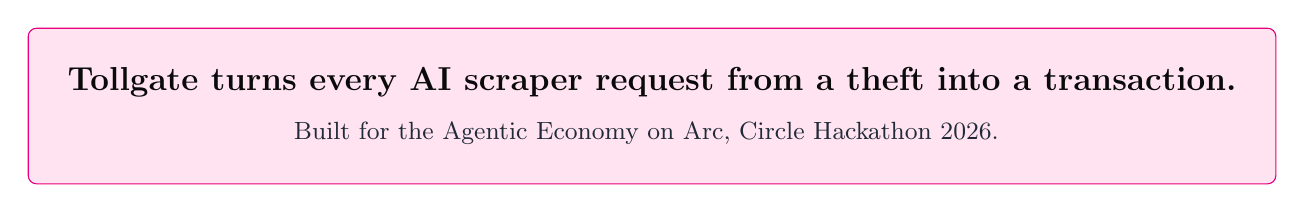
\begin{tikzpicture}
\node[draw=tollgatepink, fill=tollgatepinklight, rounded corners=3pt, minimum width=14cm, minimum height=1.5cm, align=center, inner sep=5mm] {
  \large\color{tollgateblack}\textbf{Tollgate turns every AI scraper request from a theft into a transaction.}\\[2mm]
  \small\color{tollgatecharcoal} Built for the Agentic Economy on Arc, Circle Hackathon 2026.
};
\end{tikzpicture}
\end{center}

\end{document}
